% Copyright (c) 2008-2009 solvethis
% Copyright (c) 2010-2016,2018-2019,2021 Casper Ti. Vector
% Copyright (c) 2021 Kurapica
% Public domain.
%
% 使用前请先仔细阅读 pkuthss 和 biblatex-caspervector 的文档,
% 特别是其中的 FAQ 部分和用红色强调的部分。
% 两者可在终端/命令提示符中用
%   texdoc pkuthss
%   texdoc biblatex-caspervector
% 调出。

% 为使用单页设置,可以在 [] 加入"oneside"选项 
\documentclass[UTF8,twoside]{pkuthss}

% 如果的确须要使脚注按页编号的话,可以去掉后面 footmisc 包的注释。
%\usepackage[perpage]{footmisc}

% 使用 biblatex 排版参考文献,并规定其格式(详见 biblatex-caspervector 的文档)。
% 这里按照西文文献在前,中文文献在后排序(“sorting = ecnyt”);
% 若须按照中文文献在前,西文文献在后排序,请设置“sorting = cenyt”;
% 若须按照引用顺序排序,请设置“sorting = none”。
% 若须在排序中实现更复杂的需求,请参考 biblatex-caspervector 的文档。
% biblatex-caspervector 也有一个“ugly”选项,使其更像国标格式;此外也可考虑
% 改用 style = gb7714-2015 并去掉之后两选项,详见 biblatex-gb7714-2015 的文档。
\usepackage[backend = biber, style = caspervector, utf8, sorting = none]{biblatex}
% !TEX root = ./thesis.tex
% 在此处添加需要的 packages
\usepackage{multirow}
\usepackage{makecell}
\usepackage{float}
\usepackage{tabularx}
\usepackage{tabulary}
\usepackage{amsmath}
\newcolumntype{Y}{>{\centering\arraybackslash}X}
%\newcolumntype{Z}{>{\centering\arraybackslash}m{0.2\textwidth}}

\graphicspath{{fig/}}

% 对于 linespread 值的计算过程有兴趣的同学可以参考 pkuthss.cls。
\renewcommand*{\bibfont}{\zihao{5}\linespread{1.27}\selectfont}
% 按学校要求设定参考文献列表的段间距。
\setlength{\bibitemsep}{3bp}

% 如是双盲版论文,将 \blindfalse 改为 \blindtrue。后面可用
% \ifblind 根据是否双盲来条件地启用代码(参见本文件后面部分)。
\newif\ifblind\blindfalse
% 设定文档的基本信息。
\pkuthssinfo{
	cthesisname = {本科生毕业论文}, ethesisname = {Thesis},
	thesiscover = {本科生毕业论文},
	% 长标题不用手动换行。如需强制换行,可用 \thssnl,不能用“\\”(双盲版会出错)。
	ctitle = {RustOS中的文件系统的设计与实现},
	etitle = {Design and Implementation of File System in RustOS},
	% Use ~ to add non-breaking space
	cauthor = {孙绍聪}, eauthor = {Sun Shaocong}, date = {二〇二二~年~六~月},
	studentid = {2000012977}, school = {信息科学技术学院},
	cmajor = {信息与计算科学}, emajor = {Some Major},
	% direction = {某某方向}, % 本科毕业无需填方向
	cmentor = {张杰}, ementor = {Prof.\ Somebody}, % 用于填写封面(可带教职)
  cmentornotitle = {张杰}, % 导师的姓名,用于填写评阅表
  cmentortitle = {助理教授}, % 导师的教职,用于填写评阅表
  cmentorinstitute = {计算机学院}, % 无需手动换行,控制字数<=12即可。如果字数>12,将会溢出表格
	ckeywords = {Rust,操作系统,文件系统,exFAT,页缓存,数据预取}, % 中文摘要关键词
	ekeywords = {Rust, Operating System, File System, exFAT, Page Cache,Readahead}, % 英文摘要关键词
	% 以下两项无双盲评审需求的用户可保持原状。
	% 注意 discipline/major 分别指一/二级学科。
	% blindid = {9876543210}, discipline = {某某学科}
  paperscore = {}, % 如果论文成绩须在评阅表中手动填写,此处留空即可。
}
% 载入参考文献数据库(注意不要省略“.bib”)。
\addbibresource{thesis.bib}

% 普通用户可删除此段,并相应地删除 chap/*.tex 中的
% “\pkuthssffaq % 中文测试文字。”一行。
\usepackage{color}
\def\pkuthssffaq{%
	\emph{\textcolor{red}{pkuthss 文档模版最常见问题:}}

	\texttt{\string\cite}、\texttt{\string\parencite} %
	和 \texttt{\string\supercite} 三个命令分别产生%
	未格式化的、带方括号的和上标且带方括号的引用标记:%
	\cite{test-en},\parencite{test-zh}、\supercite{test-en, test-zh}。

	若要避免章末空白页,请在调用 pkuthss 文档类时加入 \texttt{openany} 选项。

	如果编译时不出参考文献,
	请参考 \texttt{texdoc pkuthss}“问题及其解决”一章
	“上游宏包可能引起的问题”一节中关于 biber 的说明。

	因无法假定用户使用哪种方式排版表格,用户须自行保证表格字号符合学校规定。%
}

\begin{document}
	% 以下为正文之前的部分,默认不进行章节编号。
	\frontmatter
	% 此后到下一 \pagestyle 命令之前不排版页眉或页脚。
	\pagestyle{empty}
	% 自动生成封面。
	\ifblind\makeblind\else\maketitle\fi

	% 论文导师评阅表
  \cleardoublepage
	
\thispagestyle{empty}
\newgeometry{left=2cm, right=2cm, top=2.64cm, bottom=2.54cm}
\renewcommand\arraystretch{1.2}

\begin{center}
	{\songti\zihao{3}{北京大学本科毕业论文导师评阅表}}
\end{center}

%%%%%%%%%%%%%%%%%%%%%%%%%%%%%%%%%%%%%%%%%%%%%%%%%%%%%
%                                                   %
%                  请修改以下部分!                    %
%                                                   %
%%%%%%%%%%%%%%%%%%%%%%%%%%%%%%%%%%%%%%%%%%%%%%%%%%%%%

% 导师评语

\def\mentorcomment{\parbox[l]{35.88em}{
该论文研究了基于 Rust 语言开发的 Asterinas 操作系统中安全文件系统的设计与实现,对系统安全性的提升具有一定的实际意义。
 
孙绍聪同学在本研究的开展过程中,调研了 exFAT 文件系统的规范标准,实现了完整的文件系统的相关功能;为提高文件系统性能,改进了系统中页缓存的设计,增加了数据预取的功能;
为验证实现的正确性,编写了一系列单元测试并进行了集成测试;进行了一系列性能测试,验证了性能改进的有效性,并分析了现有工作的不足。
 
孙绍聪同学勤于钻研,态度端正,较好地完成了论文研究工作。毕业论文结构合理、条理清晰、写作规范、系统设计合理、实验分析有理有据,符合北京大学本科毕业论文要求。
}}


%%%%%%%%%%%%%%%%%%%%%%%%%%%%%%%%%%%%%%%%%%%%%%%%%%%%%
%                                                   %
%                   不要改动以下部分!                 %
%                                                   %
%%%%%%%%%%%%%%%%%%%%%%%%%%%%%%%%%%%%%%%%%%%%%%%%%%%%%

\def\signatureplaceholder{\parbox[l]{16em}{
  \phantom{青春大概}
  
  导师签字:\phantom{青春大概}

  \phantom{青春大概}
}}

\begin{table}[H]
\centering
\begin{tabular}{|m{2em}m{5em}m{4em}m{8em}m{6em}l|}
\hline
\multicolumn{1}{|c|}{学生姓名} & \multicolumn{1}{m{5em}|}{\authorsname}  & \multicolumn{1}{c|}{本科院系} & \multicolumn{1}{m{8em}|}{\myschool} & \multicolumn{1}{c|}{论文成绩} & \myscore \\ \cline{1-4}
\multicolumn{1}{|c|}{学生学号} & \multicolumn{1}{m{5em}|}{\mystudentid} & \multicolumn{1}{c|}{本科专业} & \multicolumn{1}{m{8em}|}{\mycmajor} & \multicolumn{1}{c|}{(等级制)} & \\ \hline
\multicolumn{1}{|c|}{\multirow{2}{*}{导师姓名}} & \multicolumn{1}{l|}{\multirow{2}{4em}{\mycmentornotitle}} & \multicolumn{1}{c|}{\multirow{2}{5em}{导师单位/ 所在学院}} & \multicolumn{1}{l|}{\multirow[]{2}{6em}{\mymentorinstitute}} & \multicolumn{1}{l|}{\multirow{2}{*}{导师职称}} & \multirow{2}{*}{\mycmentortitle}                      \\
\multicolumn{1}{|c|}{}                  & \multicolumn{1}{l|}{}                  & \multicolumn{1}{l|}{}                  & \multicolumn{1}{l|}{}                  & \multicolumn{1}{l|}{}                  &                                        \\ \hline
% \multicolumn{2}{|c|}{\multirow{2}{*}{\shortstack{论文题目\\[0.35em](中、英文)}}} & \multicolumn{4}{c|}{\multirow{2}{*}{\shortstack{\myctitle\\[0.35em]\myetitle}}}  \\
\multicolumn{1}{|c|}{\multirow{2}{*}{论文题目}} & \multicolumn{1}{c|}{中文} & \multicolumn{4}{c|}{\myctitle} \\ \cline{2-6}
\multicolumn{1}{|c|}{} & \multicolumn{1}{c|}{英文} & \multicolumn{4}{c|}{\myetitle} \\ \hline
\multicolumn{6}{|m{36.88em}|}{\center{导师评语}} \\
\multicolumn{6}{|m{36.88em}|}{\centering\kaishu{(包含对论文的性质、难度、分量、综合训练等是否符合培养目标的目的等评价)}} \\
\multicolumn{6}{|m{36.88em}|}{} \\
\multicolumn{6}{|m{36.88em}|}{{\mentorcomment}} \\
\multicolumn{6}{|m{36.88em}|}{} \\
\multicolumn{6}{|m{36.88em}|}{\hfill\signatureplaceholder} \\
\multicolumn{6}{|m{36.88em}|}{\hfill 年 \qquad\quad 月 \qquad\quad 日 \qquad\qquad\qquad} \\
\multicolumn{6}{|c|}{} \\ \hline
\end{tabular}
\end{table}

\renewcommand\arraystretch{1}
\restoregeometry



	% 版权声明。封面要求单面打印,故须新开右页。
	\cleardoublepage
	% Copyright (c) 2008-2009 solvethis
% Copyright (c) 2010-2017 Casper Ti. Vector
% All rights reserved.
%
% Redistribution and use in source and binary forms, with or without
% modification, are permitted provided that the following conditions are
% met:
%
% * Redistributions of source code must retain the above copyright notice,
%   this list of conditions and the following disclaimer.
% * Redistributions in binary form must reproduce the above copyright
%   notice, this list of conditions and the following disclaimer in the
%   documentation and/or other materials provided with the distribution.
% * Neither the name of Peking University nor the names of its contributors
%   may be used to endorse or promote products derived from this software
%   without specific prior written permission.
%
% THIS SOFTWARE IS PROVIDED BY THE COPYRIGHT HOLDERS AND CONTRIBUTORS "AS
% IS" AND ANY EXPRESS OR IMPLIED WARRANTIES, INCLUDING, BUT NOT LIMITED TO,
% THE IMPLIED WARRANTIES OF MERCHANTABILITY AND FITNESS FOR A PARTICULAR
% PURPOSE ARE DISCLAIMED. IN NO EVENT SHALL THE COPYRIGHT HOLDER OR
% CONTRIBUTORS BE LIABLE FOR ANY DIRECT, INDIRECT, INCIDENTAL, SPECIAL,
% EXEMPLARY, OR CONSEQUENTIAL DAMAGES (INCLUDING, BUT NOT LIMITED TO,
% PROCUREMENT OF SUBSTITUTE GOODS OR SERVICES; LOSS OF USE, DATA, OR
% PROFITS; OR BUSINESS INTERRUPTION) HOWEVER CAUSED AND ON ANY THEORY OF
% LIABILITY, WHETHER IN CONTRACT, STRICT LIABILITY, OR TORT (INCLUDING
% NEGLIGENCE OR OTHERWISE) ARISING IN ANY WAY OUT OF THE USE OF THIS
% SOFTWARE, EVEN IF ADVISED OF THE POSSIBILITY OF SUCH DAMAGE.

% 此处不用 \specialchap,因为学校要求目录不包括其自己及其之前的内容。
\chapter*{版权声明}
% 综合学校的书面要求及 Word 模版来看,版权声明页不用加页眉、页脚。
\thispagestyle{empty}

任何收存和保管本论文各种版本的单位和个人,
未经本论文作者同意,不得将本论文转借他人,
亦不得随意复制、抄录、拍照或以任何方式传播。
否则,引起有碍作者著作权之问题,将可能承担法律责任。

% 若须排版二维码,请将二维码图片重命名为“barcode”,
% 转为合适的图片格式,并放在当前目录下,然后去掉下面 2 行的注释。
%\vfill\noindent
%\includegraphics[height = 5em]{barcode}

% vim:ts=4:sw=4


	% 此后到下一 \pagestyle 命令之前正常排版页眉和页脚。
	\cleardoublepage
	\pagestyle{plain}
  
	% 重置页码计数器,用大写罗马数字排版此部分页码。
	\setcounter{page}{0}
	\pagenumbering{Roman}
	% 中西文摘要。
	% Copyright (c) 2014,2016,2021 Casper Ti. Vector
% Public domain.

\begin{cabstract}
	%\pkuthssffaq % 中文测试文字
	摘要。
\end{cabstract}

\ifblind\begin{beabstract}\else\begin{eabstract}\fi
	Test of the English abstract.
\ifblind\end{beabstract}\else\end{eabstract}\fi

% vim:ts=4:sw=4

	% 自动生成目录。
	\tableofcontents

	% 以下为正文部分,默认要进行章节编号。
	\mainmatter
	% 各章节。
	% Copyright (c) 2014,2016,2018 Casper Ti. Vector
% Public domain.

\chapter{引言}

\section{操作系统安全性的重要性}
信息安全\parencite{SOOMRO2016215}是当今数字化社会中至关重要的一个领域,关系到保护数据、系统和网络免受未经授权的访问、使用、泄露、破坏或干扰等方方面面。
在信息安全领域,操作系统的安全性是一个核心议题,因为操作系统作为计算机系统的基础软件,直接影响整个系统的安全性。

就像著名的计算机科学家安德鲁·坦宁斯(Andrew Tanenbaum)在其著作《现代操作系统》\parencite{tanenbaum2014modern}中指出:“操作系统的安全性是整个系统安全的基石。” 
但传统的操作系统,尤其是基于 C/C++ 的操作系统,由于其对内存管理等方面的处理特性,或多或少地存在着一定的安全隐患。
这些安全隐患可能被恶意用户或恶意软件利用,从而导致系统遭受攻击,出现数据泄露或服务中断等问题。

因此,如何提高操作系统的安全性,是当今信息科学的重要研究课题。

\section{Rust语言在操作系统开发中的优势}
Rust 语言\parencite{matsakis2014rust}作为一种系统编程语言,旨在实现“安全、并发、实用”的设计目标。
其最显著特征在于其所有权系统,这一系统在编译时期能够检测并预防内存安全问题,如空指针解引用和缓冲区溢出等常见内存错误。
相比于 C/C++ 在这些问题上需要开发者自行处理,Rust 语言的静态检查能够自动发现并解决这些问题,从而显著提高了代码的安全性。

除了内存安全方面的优势,Rust 还利用其独特的特性如模式匹配、枚举类型等简化了对函数返回值的处理,
使得程序中的错误处理逻辑更加优雅。
这种简化不仅减轻了开发者的负担,还有助于提高代码的可读性和可维护性,从而提升了开发效率。
在操作系统的开发中更是显得尤为重要。

因此,将 Rust 语言应用于操作系统开发,有望提高操作系统的安全性和可靠性。
Rust 通过其内存安全保证和优雅的错误处理机制,为操作系统开发提供了一种更加安全、高效的编程方式。
同时,Rust 语言的高性能特性和高开发效率也使其成为开发操作系统的理想选择,
能够在保证系统性能的同时提升开发效率,为构建更安全、更可靠的操作系统奠定坚实基础。

\section{本研究的目标和重要性}
本研究立足于使用 Rust 编写的新兴操作系统 Asterinas\parencite{Asterinas},旨在完善其文件系统实现。
我们为 Asterinas 新增了 exFAT 文件系统\parencite{exFAT}\parencite{exFAT1}\parencite{exFAT2}的实现,并利用 Rust 语言的特性进行定制化设计。此外,
本研究还为其文件系统的页缓存\parencite{tanenbaum2014modern}\parencite{ostep}\parencite{bovet2005understanding}增加了
数据预取\parencite{readahead}\parencite{sequential_prefetching}的功能,可以很大程度上改善页缓存在顺序读写模式下的
性能表现,有助于进一步提高文件系统的性能,这一点也在测试中得到了证实。

本文剩余部分按下述结构进行组织:
\begin{itemize}
    \item 第二章介绍本工作的相关背景,包括 Rust 语言、exFAT 文件系统和页缓存数据预取。
    \item 第三章阐述 exFAT 文件系统的具体设计实现。
    \item 第四章阐述页缓存中数据预取的具体设计实现。
    \item 第五章针对实现的 exFAT 文件系统进行了正确性测试,主要包括单元测试和集成测试。
    \item 第六章针对实现的 exFAT 文件系统进行了性能测试,并与 Linux 中的实现进行了比较。
    \item 第七章对文章进行总结并提出未来可能的工作方向。
\end{itemize}



%\newpage
%偶数页的风格是这样的。

% vim:ts=4:sw=4

	% Copyright (c) 2014,2016 Casper Ti. Vector
% Public domain.

\chapter{背景}
%\pkuthssffaq % 中文测试文字。
\section{exFTA文件系统}
exFAT (Extended File Allocation Table)\parencite{exFAT} 是由微软公司开发的一种文件系统,
专为闪存存储,如USB闪存驱动器、SD卡和CF卡等设计。作为FAT32的后继文件系统,
exFAT 主要解决了FAT32在处理大文件和大容量存储设备上的限制。具体来说,
exFAT 文件系统使用64位来描述文件大小,从而支持依赖于非常大的文件的应用程序;
exFAT 文件系统还允许最大32MB的簇,有效地支持了非常大的存储设备。

exFAT文件系统在存储设备上的分区可以划分为三个主要部分:启动区、FAT区和数据区,如图??所示。
启动区包含超级块和后备超级块。
超级块(Superblock)中包含文件系统的基本信息,如扇区和簇的大小、FAT区和数据区的位置,、根目录所在簇等。
超级块一般位于存储设备上 exFAT 分区的起始位置,会在exFAT打开时被读取。
利用超级块中的信息,操作系统可以读取文件分配表并初始化根目录。
超级块对 exFAT 文件系统非常重要,因此还会安排一个后备超级块(Backup Superblock),以应对超级块损坏的情况。
如果超级块和后备超级块都损坏了,exFTA 文件系统将无法被挂载。

exFAT 将数据区里存储文件的部分(一般被称为簇堆,Cluster Heap)划分为一系列的簇(Cluster),
一个簇一般包含若干扇区。
扇区是存储设备的最小读写单元,而簇是文件分配的最小单元,即块设备上逻辑存储的基本单位。
作为FAT文件系统家族中的一员, exFAT 也使用文件分配表(FAT,File Allocation Table)来组织文件。
文件分配表描述了簇和文件内容之间链接关系,位于启动区之后的FAT区。
一个文件可能由若干簇组成,这些簇组成了一个簇链。
对于使用FAT的分配方式,文件分配表中维护了当前簇的下一个簇的编号。
这种组织结构类似链表,如果将一个文件中的一系列簇视作一个链表,
文件分配表中的条目相当于链表结构中的 Next 指针。
在读取某个文件时,通过查找文件分配表可以依次找到文件在磁盘上对应的各个簇的编号,从而访问文件的内容。
出于某些历史上的原因, exFAT 的簇编号从 2 开始,也就是说,假设数据区一共包括 $ N $ 个簇,第一个簇的编号是 2,
最后一个簇的编号是 $ N + 1 $。若从文件分配表中得到某个合法的簇编号 $ C $,该簇的物理编号是 $ C - 2 $。

数据区则是用于存储用户的文件和文件夹的区域,exFAT 文件系统内的所有文件和文件夹(包括根目录和系统文件)
的数据都存储在这个区域,并使用文件分配表来进行组织。
exFAT使用目录树结构来管理存于簇堆中的文件系统结构和文件。
在目录树中,父目录与子目录之间存在一对多的关系。
超级块中记录了文件系统的根目录所在簇,所有其他的目录都以单链方式从根目录派生。
每个目录由一系列目录项(Directory entry,在本文中简称为Dentry)组成,exFAT中的单个目录项的大小固定为32字节。
事实上,exFAT内的目录文件的文件内容就是一系列目录项。
一个或多个目录项可以组成一个目录项集(Directory entry set,在本文中简称为Dentry set),
用于描述文件系统结构,子目录或文件。

每一个有效的目录项可以按照属于主目录项或次目录项、属于关键目录项还是可选目录项分为四类。
每一个目录项集都是由一个主目录项和一系列次目录项组成,主目录项中会指明相关联的次目录项的个数。
关键主目录项包含一些对于exFAT文件系统的正确管理至关重要的信息,所有这种类型的目录项都应当被实现。
可选主目录项的实现是可选的,这类目录项的作用是辅助管理文件系统,我们的实现中暂时并未支持这类目录项。
关键次目录项包含管理其所在目录项集的关键信息,虽然对任何关键次目录项的支持是可选的,但一个未识别的
关键目录项会使整个目录项集无法识别,我们的实现还是支持了exFAT标准中出现的所有关键次目录项。
可选次目录项的实现也是可选的,一个目录项集中出现的未识别的可选次目录项可以被忽略。
除此之外,exFAT 还定义了两种无效的目录项:未使用的目录项(Unused)和被删除的目录项(Deleted)。
表\ref{tab:dentry}中列出了我们的实现中主要的Dentry类型。
\begin{table}[h]
    \centering
    \begin{tabularx}{\textwidth}{|c|c|Y|}
    \hline
    Dentry类型 & 种类 & 描述 \\
    \hline
    Bitmap & 关键主目录项 & 与系统文件 Bitmap 关联的目录项,位于根目录中,没有次目录项,Bitmap用于跟踪磁盘上的空闲簇和已分配簇\\
    \hline
    Upcase Table & 关键主目录项 & 与系统文件大写转换表(Upcase Table)关联的目录项,位于根目录中,没有次目录项,大写转换表用于支持exFAT对大小写不敏感的特性\\
    \hline
    File & 关键主目录项 & 描述文件和目录的信息,合法的 File 目录项后会跟着一个 Stream 目录项和至少一个 Name 目录项\\
    \hline
    Stream & 关键次目录项 & 补充描述文件和目录的信息,紧跟 File 目录项出现\\
    \hline
    Name & 关键次目录项 & 记录相关文件和目录的名称,紧跟 Stream 目录项出现\\
    \hline
    Vendor Extension & 可选次目录项 & 文件供应商自定义目录项,只能出现在 Stream 和 Name 目录项之后\\
    \hline
    Vendor Allocation & 可选次目录项 & 文件供应商自定义目录项,只能出现在 Stream 和 Name 目录项之后\\
    \hline
    Unused & - & 未使用的目录项,只能出现在所在目录的末尾\\
    \hline
    Deleted & - & 被删除的目录项\\
    \hline
    \end{tabularx}
    \caption{Dentry 类型}
    \label{tab:dentry}
\end{table}



\section{页缓存及数据预取}
页缓存(Page Cache)是一种计算机系统常用的用于加速数据访问的技术。利用应用程序访问数据的局部性特点,
通过将常用的文件的数据缓存至内存,从而加速对文件数据的访问。数据预取(Readahead)则是一种预测性的技术,
它根据应用过去的访问模式来预测未来可能需要的数据,并提前从磁盘上读取这些数据到页缓存中。当这些数据
真正被访问时,它们已经在内存中可用,从而避免了磁盘访问的延迟。
因此,对于有明显访问模式的应用(如顺序访问),数据预取可以显著提高应用程序的性能。
本文主要关注顺序访问模式,为Asterinas的页缓存实现了数据预取。

% vim:ts=4:sw=4

	% Copyright (c) 2014,2016,2018 Casper Ti. Vector
% Public domain.

\chapter{exFAT文件系统的设计与实现}
%\pkuthssffaq % 中文测试文字。
本研究实现的 exFAT 文件系统可以划分成以下几个相对独立模块:文件系统的中枢部分、FAT表及文件的分配与访问、目录的解析、
大写转换表、Bitmap、索引节点实现,各个模块之间存在交互。
其中文件系统的中枢部分是文件系统的核心,里面包括了exFAT的所有组件的实例,
并对外提供和整个文件系统相关的接口。
索引节点(Index node,本文中简称为 Inode)实现了和单个文件或文件夹相关的功能,对外提供和单个文件或文件夹操作相关的接口。
其他部分不对外提供接口,仅在文件系统内部使用。
图\ref{fig:exfat_arch}是我们实现的exFTA的总架构图。

\begin{figure}[h]
    \centering
    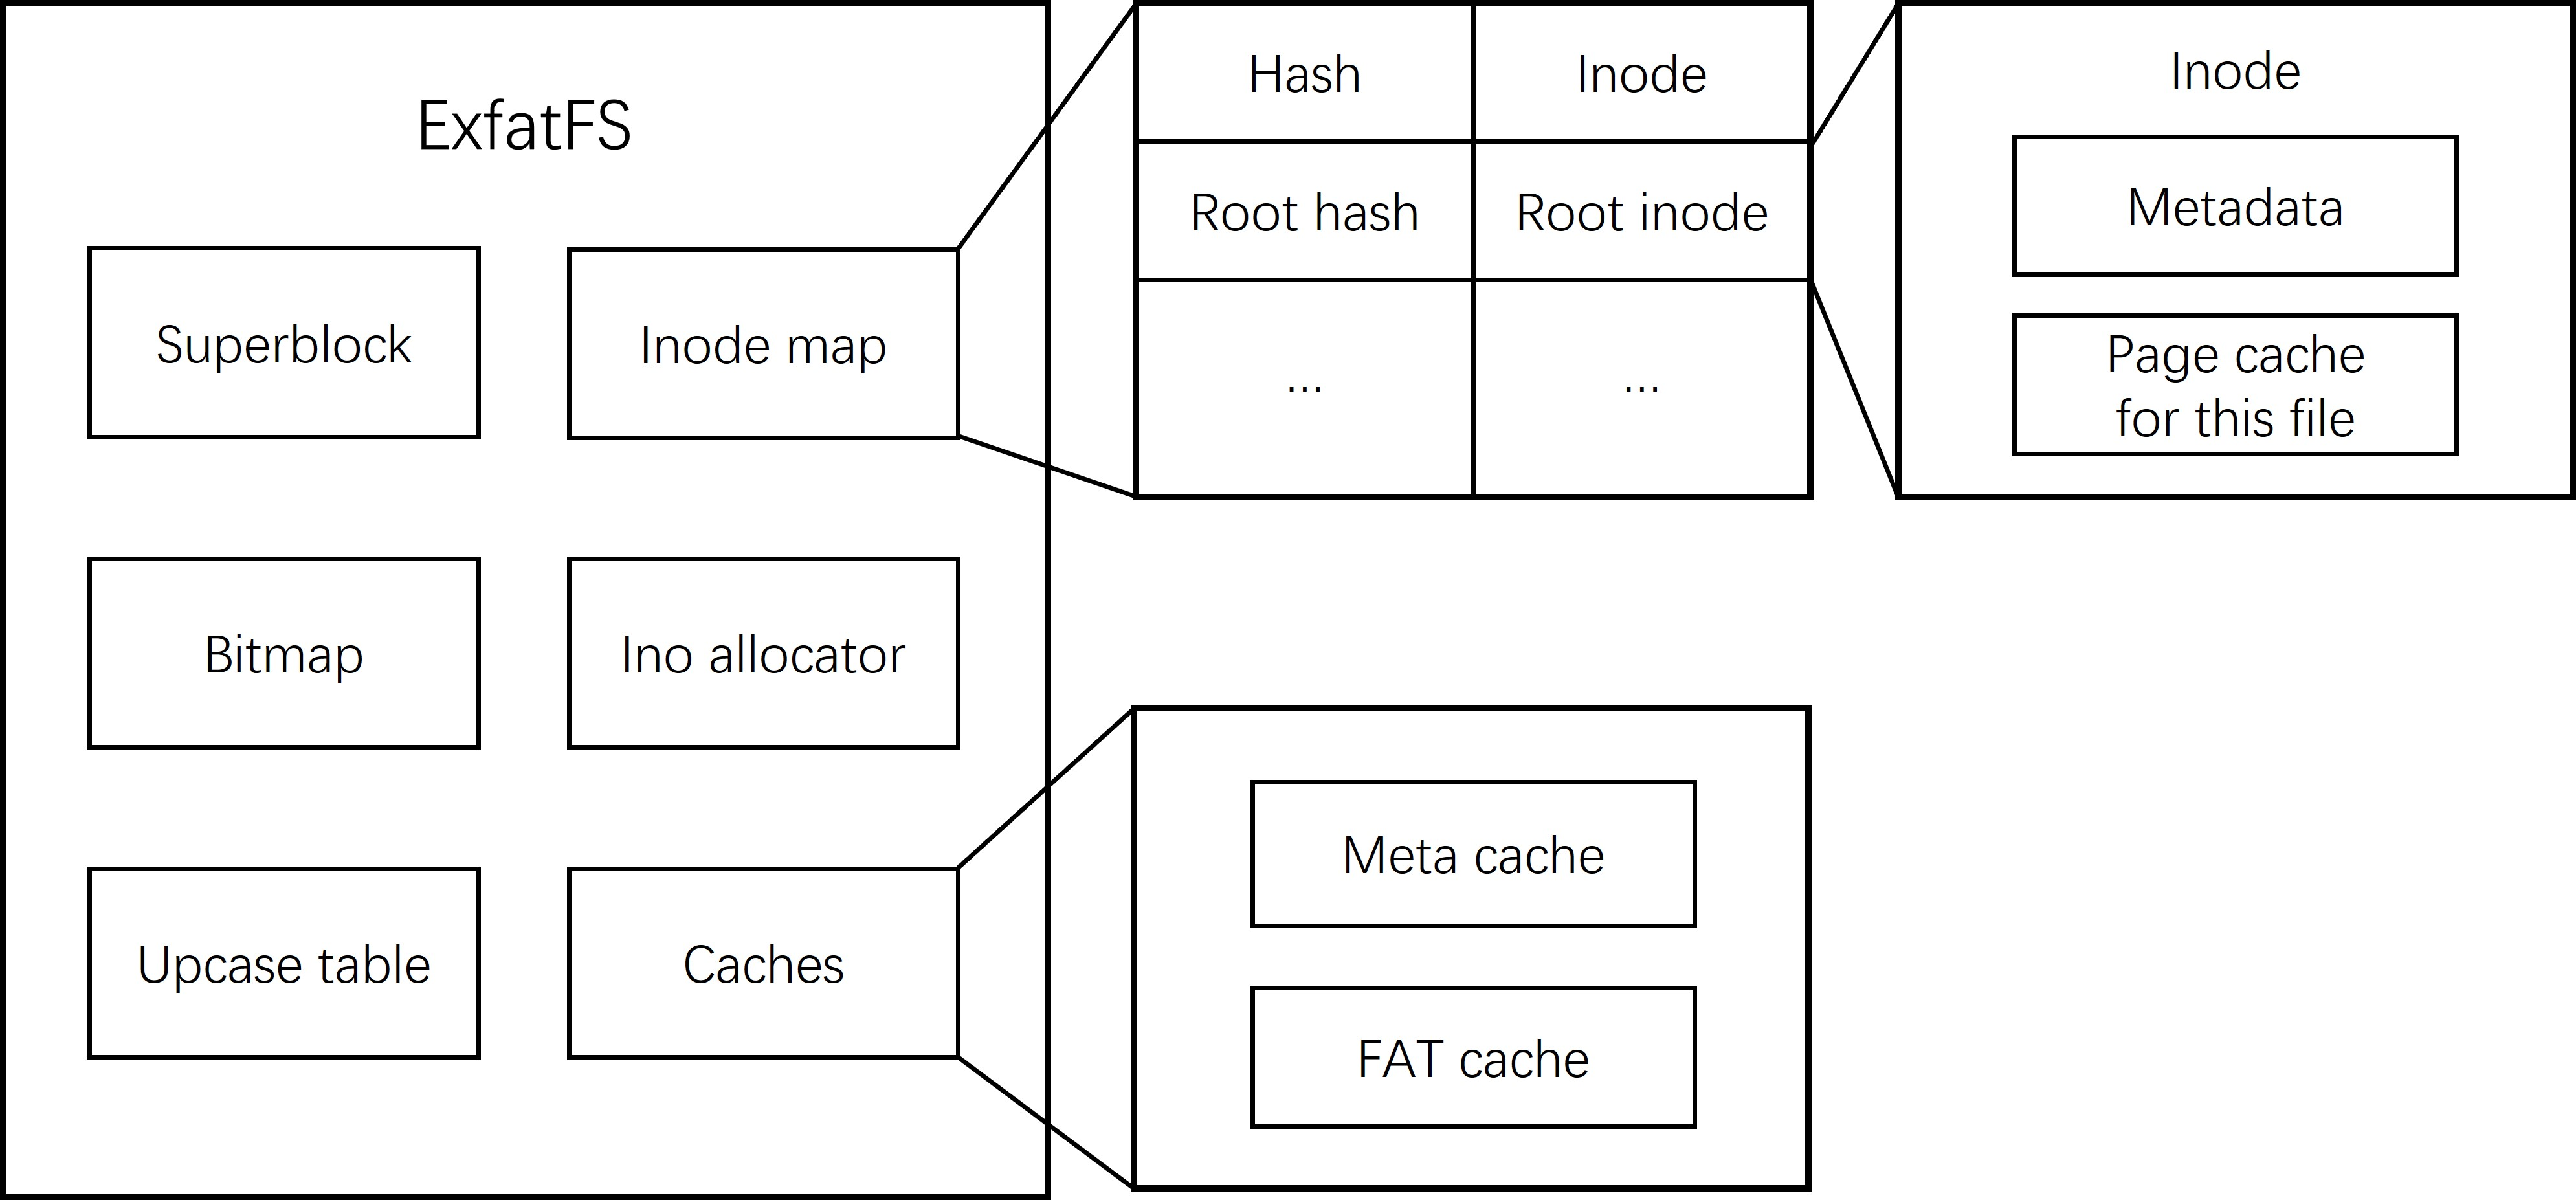
\includegraphics[width=1.0\textwidth]{chap3_exfat_arch.jpg}
    \caption{exFAT总架构}
    \label{fig:exfat_arch}
\end{figure}
\section{文件系统的中枢部分}
文件系统的中枢部分被实现为图\ref{fig:exfat_arch}中的结构体 ExfatFS,这个结构体会在 exFTA 被挂载时创建,伴随 exFAT 直至其被取消挂载。
ExfatFS 中的首要功能就是挂载 exFAT 文件系统。
exFAT 被挂载时会首先从块设备上读取超级块,若发现位于起始位置的超级块受损,
系统会尝试读取后备超级块。当系统读取到正确的超级块后,可以从其中获取文件系统的基本信息,
包括扇区和簇的大小和数量、根目录所在簇、FAT区的起始扇区和数据区的起始扇区。
随后,系统会根据根目录所在簇打开根目录,建立根目录的索引节点(Root inode)。
根目录的 Inode 被分配到 Inode 编号是 1,这也是最小的 Inode 编号。
接着,系统会在根目录中寻找 Bitmap 目录项和 Upcase Table 目录项,分别初始化 Bitmap 和大写转换表。
至此,exFAT 文件系统挂载完成。

ExfatFS 作为文件系统的中枢部分,负责管理所有打开的Inode和分配Inode编号(Inode number,本文中简称Ino)。
每打开一个新的Inode,ExfatFS 的Ino分配器(Ino allocator)会为其分配一个新的编号。
Ino分配器被实现为一个支持原子操作的64位无符号数,维护下一个要分配的 Ino。
当需要分配新的Ino时,Ino分配器会进行自增,并返回自增前的值作为分配结果。
ExfatFS 使用一个 HashMap 管理打开的Inode,如图\ref{fig:exfat_arch}中的Inode map所示。
使用 HashMap 的目的是能通过文件相关信息计算出哈希值,从而直接找到对应的Inode。
哈希值的选择应该满足在整个 exFAT 文件系统中唯一,故不能使用文件名的字符串哈希做哈希值。
完整路径名的字符串哈希是一个可行的选择,但可能存在潜在的哈希值碰撞的情况。
我们的设计中采用了另一种计算哈希值的方式,如式\ref{eq:hash}所示,使用某文件对应的目录项集的主目录项的位置来计算哈希值
(唯一的特例是根目录,根目录不存在关联的目录项),这种计算方式显然可确保唯一性,而且也不存在碰撞的可能。
\begin{equation}\label{eq:hash}
    hash(inode) = 
    \begin{cases}
        root\_hash & \text{root inode} \\
        (pos.cluster\_id \ll 32) \text{ }|\text{ } pos.offset & \text{other inode}
    \end{cases}
\end{equation}
在元数据管理方面,ExfatFS 使用了两个 Cache 来缓存与管理 exFAT 中涉及的元数据。
第一个 Cache (Meta cache)是一个普通的页缓存,按页粒度缓存 exFAT 中元数据相关的页面,
这可能包括FAT区的页面、系统文件 Bitmap 和大写转换表中的页面等。
为了方便访问FAT表,我们还使用了另一个 Cache,第二个 Cache (FAT cache)是一个基于LRU的 Cache,
缓存粒度是具体的FAT表项,Cache 中的每个条目都代表单个FAT映射。

\section{FAT表及文件的分配与访问}\label{sec:FAT}
exFTA文件系统的所有文件和目录数据都存储在位于数据区的簇堆中,簇堆是一系列的簇的集合。
数据的位置可以通过一个二元组(簇的编号 Cluster id,簇内偏置 offset)唯一确定。

exFAT允许的文件分配方式有两种:连续分配和使用FAT表分配。
连续分配不使用FAT表,使用这种分配方式的文件会在目录项中给出文件起始簇的编号和文件的大小,
访问文件内容的过程无需查找FAT表。
使用FAT表分配的方式将文件内容组织成一系列的簇链,通过FAT表可以获取当前簇的下一个簇编号,
访问文件内容的过程需要从文件起始簇不断通过查询FAT表到达访问的位置。
exFAT引入连续分配模式的目的主要是为了加速文件内寻址的过程。
很显然,只要存储空间足够,我们总可以使用FAT表进行文件的分配和组织,
而连续分配需要保证存在足够大的连续空闲空间,这一点可以通过查找 Bitmap 获得。
我们实现的exFAT文件系统的分配逻辑可以总结为:优先连续分配模式,优先不改变分配模式。
对于一个从零分配的文件,我们会首先尝试连续分配,若此时的空闲簇不满足连续分配的条件,则转向使用FAT表的分配模式。
至于扩展一个已分配文件的大小,若该文件的分配方式是使用FAT表分配,则保持分配方式不变即可;
若该文件的分配方式是连续分配,则会首先尝试继续使用连续分配,从文件末尾处扩展文件,如果无法延续,
则转向使用FAT表的分配模式并为已分配的部分补充填写FAT表。

\begin{figure}[h]
    \centering
    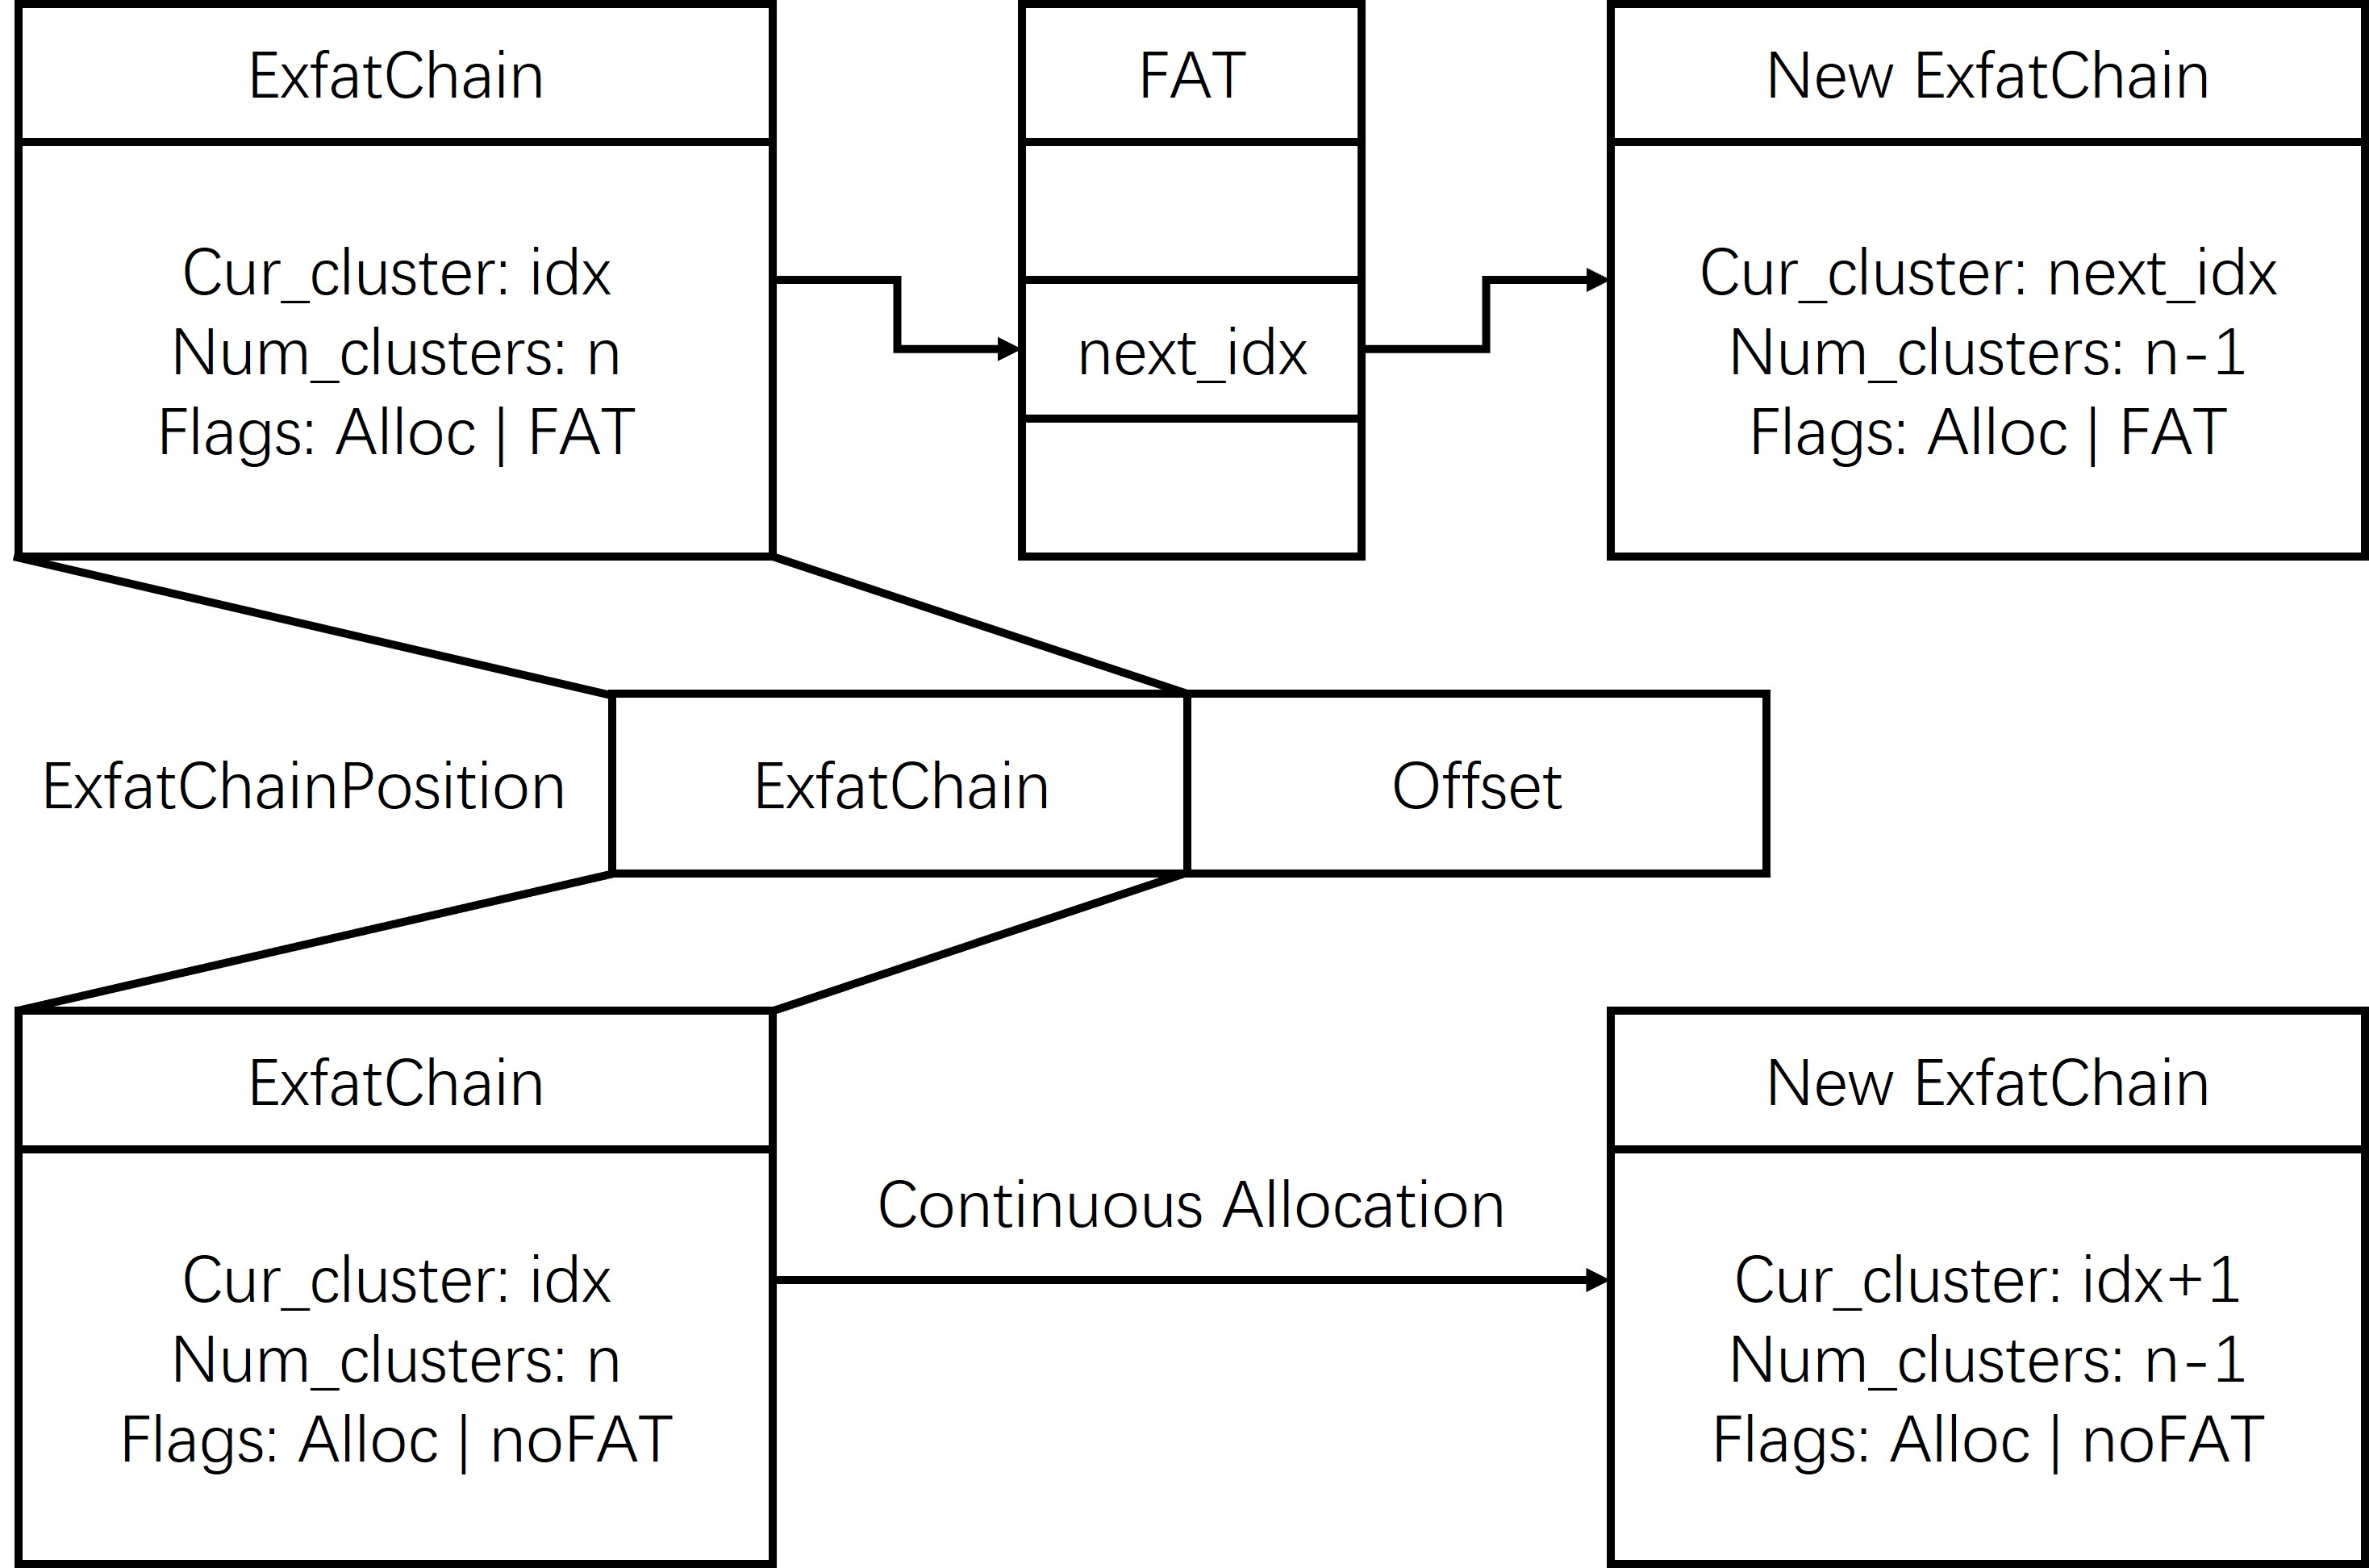
\includegraphics[width=0.8\textwidth]{chap3_cluster_chain.jpg}
    \caption{ExfatChain 寻址过程}
    \label{fig:cluster_chain}
\end{figure}

综合以上,我们把簇链抽象成 ExfatChain 结构体,使用一个二元组 (ExfatChain,Offset) 来描述数据的具体位置。
ExfatChain 结构体包含了当前簇的编号、后续合法簇的数量、文件分配方式等信息。
图\ref{fig:cluster_chain}展示了在不同分匹配模式下,使用 ExfatChain 结构进行寻址过程。
图\ref{fig:index_in_file}则展示了一个完整的数据访问过程。当应用需要访问存储设备上文件内的某个 $ offset $ 时,
通过文件的Inode内 start\_chain 字段获得文件起始簇 start\_cluster 。
访问目标的位置位于从 start\_cluster 簇开始的第 $ offset \text{ }\%\text{ } cluster\_size $ 个簇 target\_cluster 内,
簇内偏置为 $ offset \text{ }/\text{ } cluster\_size $ 。
按照图\ref{fig:cluster_chain}在描述的方式,通过文件的分配模式决定是否使用FAT表,我们可以计算出 target\_cluster 的编号。
至此,我们得到了访问目标在存储设备上的位置,访问底层设备或页缓存即可获得需要访问的数据。

\begin{figure}[h]
    \centering
    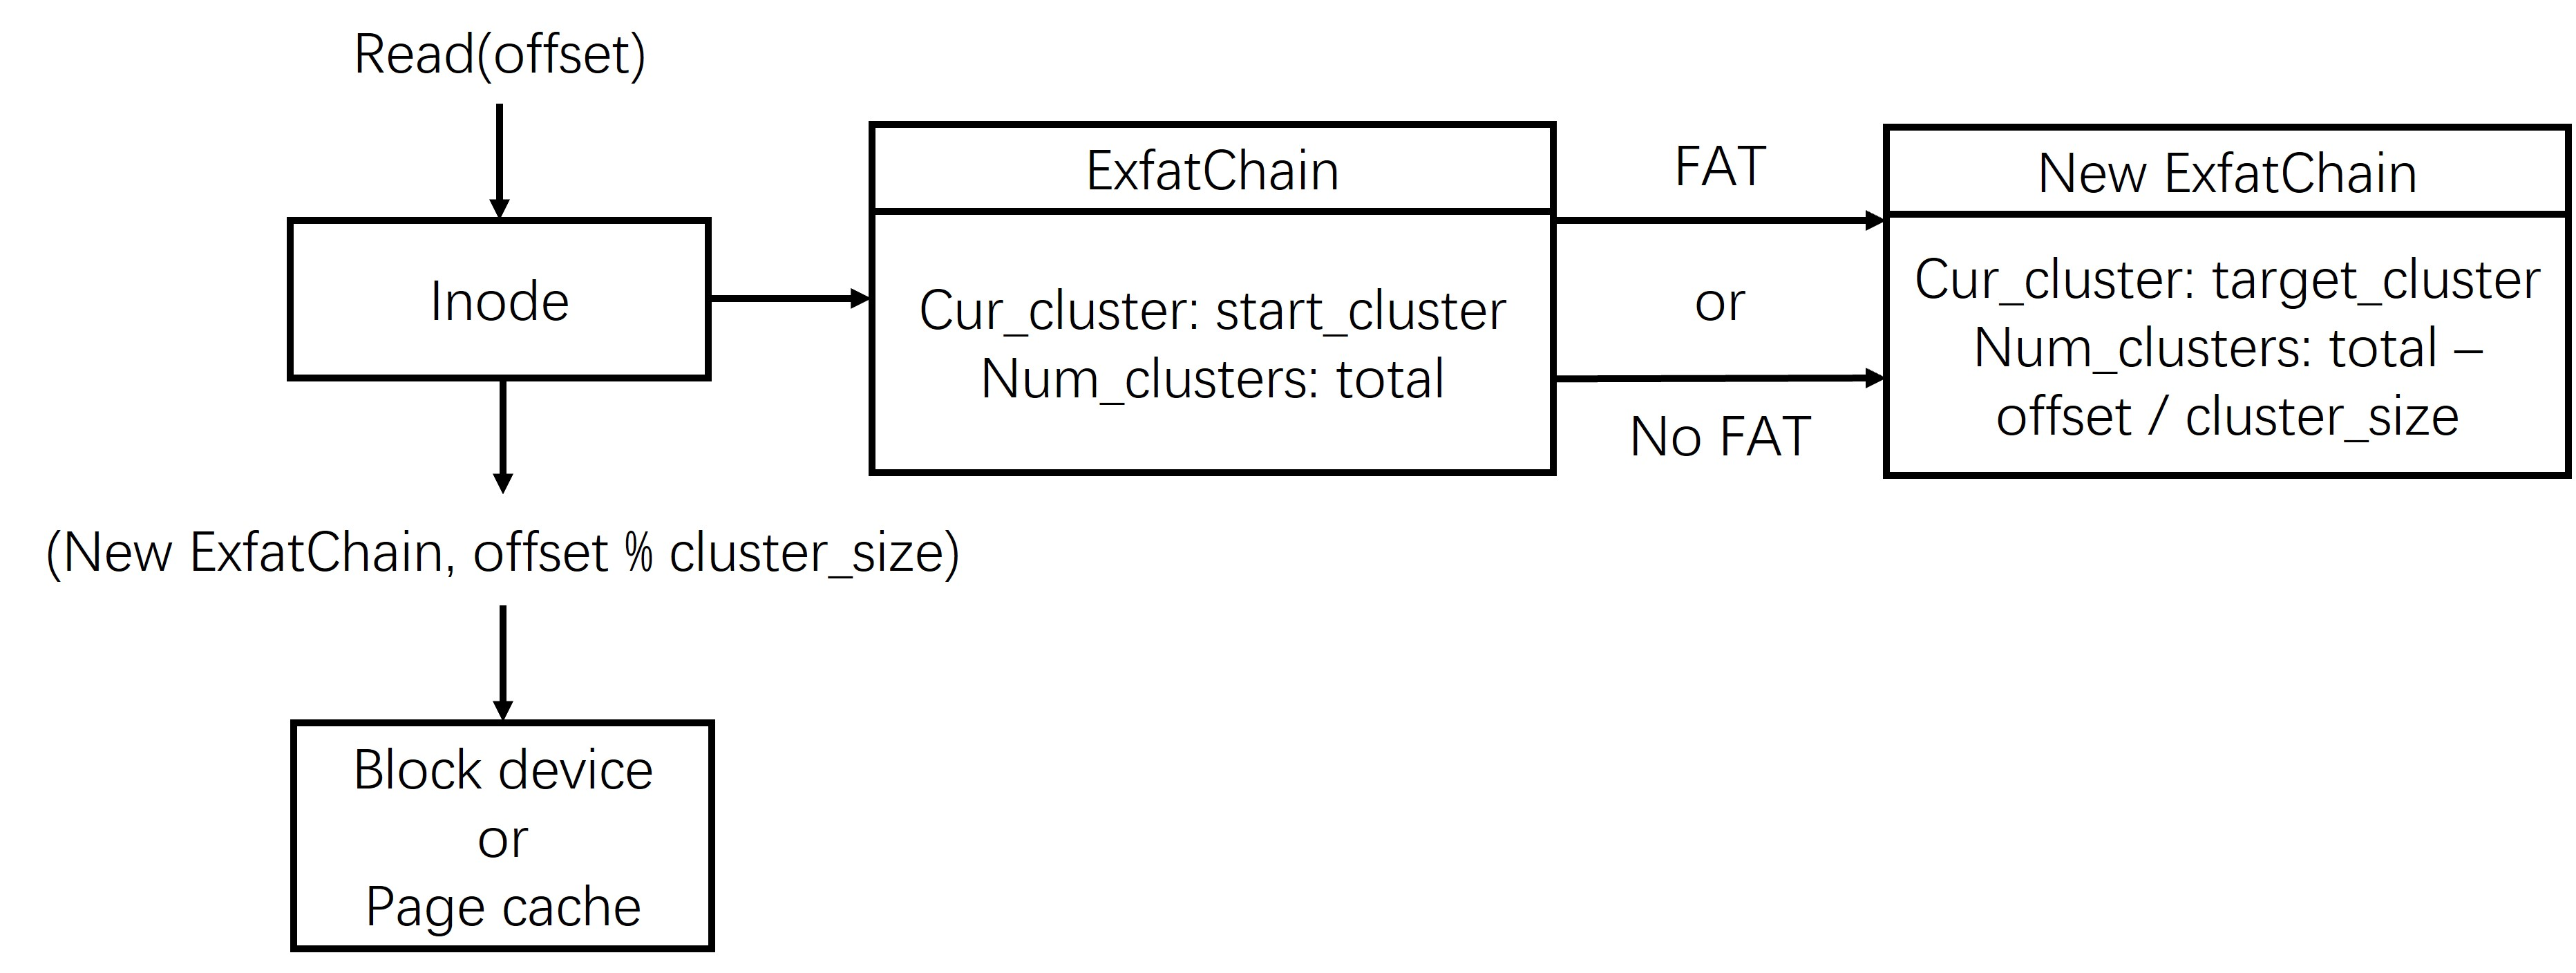
\includegraphics[width=1.0\textwidth]{chap3_index_in_file.jpg}
    \caption{文件数据访问过程}
    \label{fig:index_in_file}
\end{figure}

\section{目录的解析}\label{sec:dentry}
目录文件的文件内容是一系列目录项,一组目录项可以组成目录项集。
目录项集是对exFAT文件系统内的具体文件的抽象,exFTA内的除了根目录的每个文件都对应着一个目录项集。
这里先不讨论与大写转换表和 Bitmap 这两个特殊的系统文件对应的目录项集。
文件对应的目录项集被存储为其父目录内一组逻辑连续的目录项,分布在父目录的一段连续的逻辑地址上。
正如第二章指出的,每个目录项集由一个主目录项和一系列次目录项组成,主目录项中会指明相关联的次目录项的个数。
于是,当我们遍历一个目录的内容时,只要找到了一个主目录项,之后便可根据主目录项的信息完整的读出整个目录项集。

\begin{figure}[h]
    \centering
    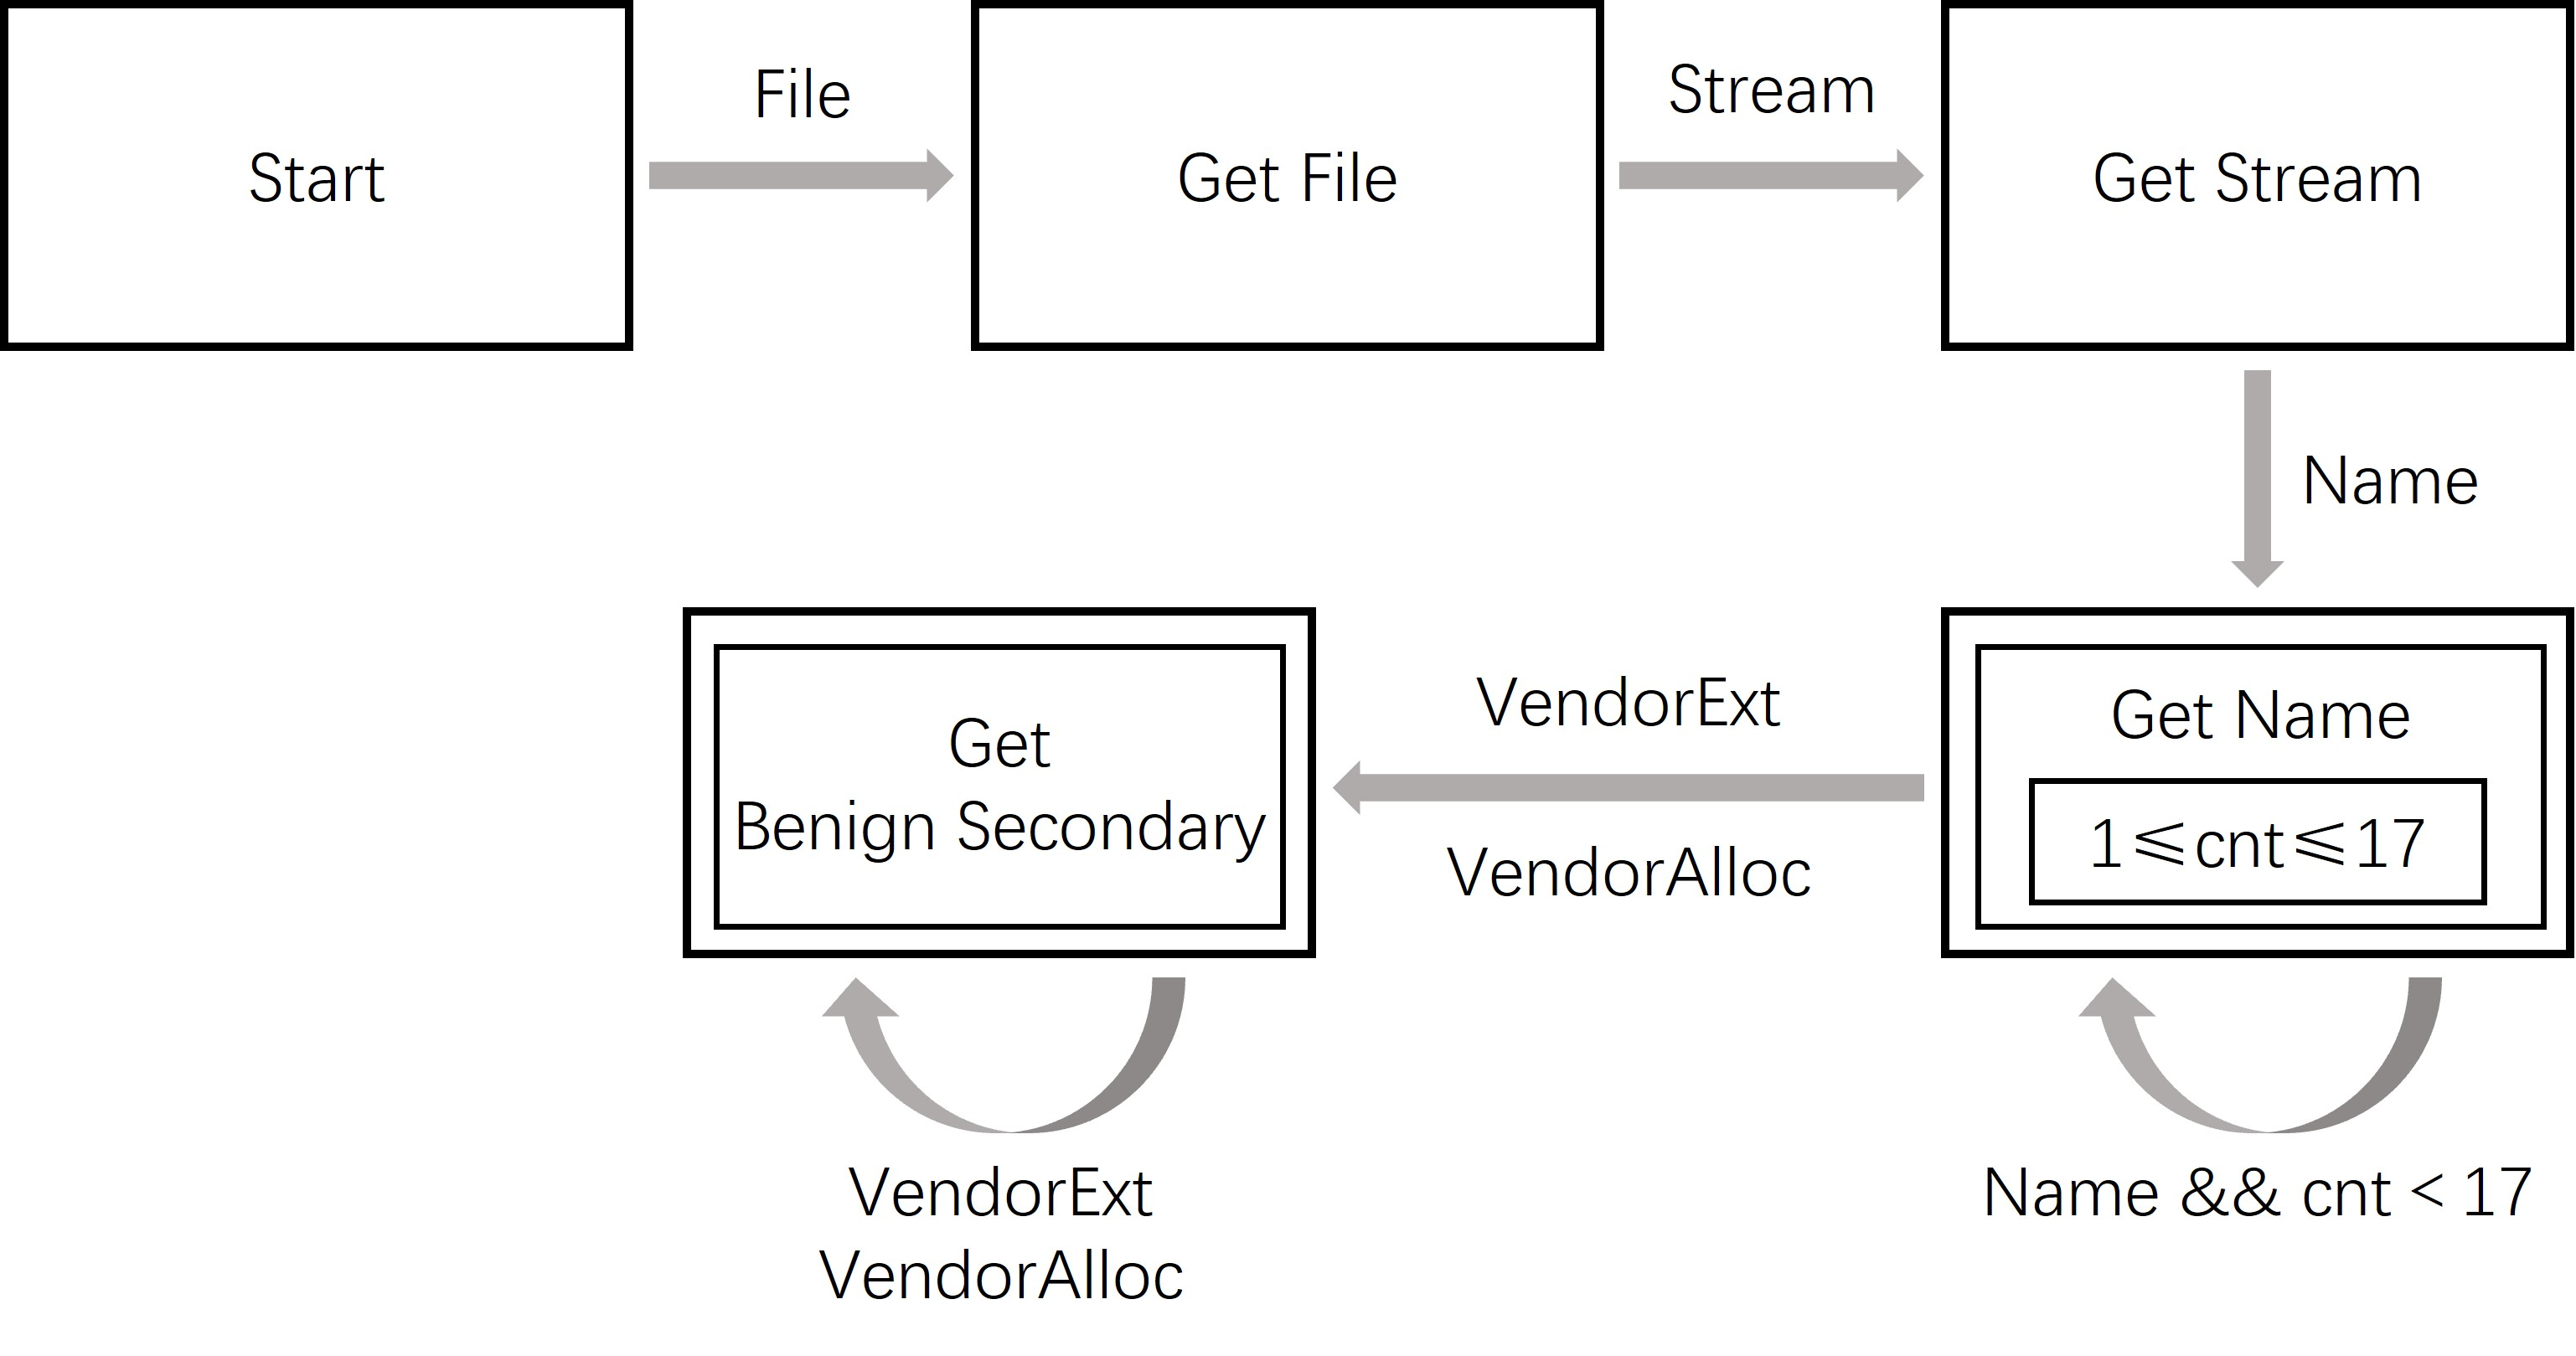
\includegraphics[width=0.8\textwidth]{chap3_dentry_state.jpg}
    \caption{目录项集解析状态机}
    \label{fig:dentry_state}
\end{figure}

读出目录项集后,需要检验其合法性。
从主目录项开始,按顺序遍历一个合法的目录项集的过程可以用一个有限状态机表示,如图\ref{fig:dentry_state}所示。
初始状态是 Start,每遇到一个新的目录项,便会根据目录项的类型转移到新状态,图中未出现的转移都是不合法的。
其中状态 GetName 包括一个参数 $ cnt $,表示当前状态下读取到的 Name 目录项的个数。
$ cnt $ 在刚进入 GetName 状态时的初始值是1,在此状态下每读到一个新的 Name 目录项,$ cnt $ 的值就增加1。
合法的终止状态包括 GetName($ 1 \leq cnt \leq max\_cnt = 17 $) 和 GetBenignSecondary。 
读出整个目录项集后,需要按顺序遍历目录项集并更新相应状态,
若遍历后到达一个合法的终止状态,则这个目录项集是合法的。


\section{大写转换表与 Bitmap}
大写转换表和 Bitmap 都是特殊的系统文件,位于根目录中,对应的目录项集均只包含一条主目录项。

大写转换表用于支持exFAT对大小写不敏感的特性,这主要是为了保证文件系统的跨平台兼容性。
exFAT的标准规定在比较两个文件名时,只要将他们都用大写转换表转换成大写后相同,就认为他们是相同的。
所以,exFAT不允许同一文件夹下存在仅通过大小写区分的文件名。
值得注意的一点是,虽然exFAT比较文件名时会使用大写转换表将文件名转化成大写,exFAT在存储文件名时
还是按照用户提供的形式存储,使用文件管理器查看时也会显示未经转换的文件名。

Bitmap 用于跟踪磁盘上的空闲簇和已分配簇,数据区中的每一个簇对应 Bitmap 中的一位,
在 Bitmap 中分别用0和1表示相应的簇未分配和已分配。
仍然需要注意的是,exFAT 中的簇的编号从2开始,而 Bitmap中的第 $ i $ 个比特代表第 $ i $ 个簇的分配状态。
故编号为 $ C $ 的簇对应 Bitmap 中的下标为 $ C - 2 $ 的比特。

\section{索引节点的实现}
索引节点,即Inode,是文件系统里最关键的组件。
作为文件在内存中的抽象,大部分和具体文件相关的系统调用都是通过 Inode 实现的。
在小节\ref{sec:FAT}和小节\ref{sec:dentry}中分别介绍了如何访问文件的内容以及如何解析目录,
在此基础上可以实现和具体文件相关的所有操作。

\begin{figure}[h]
    \centering
    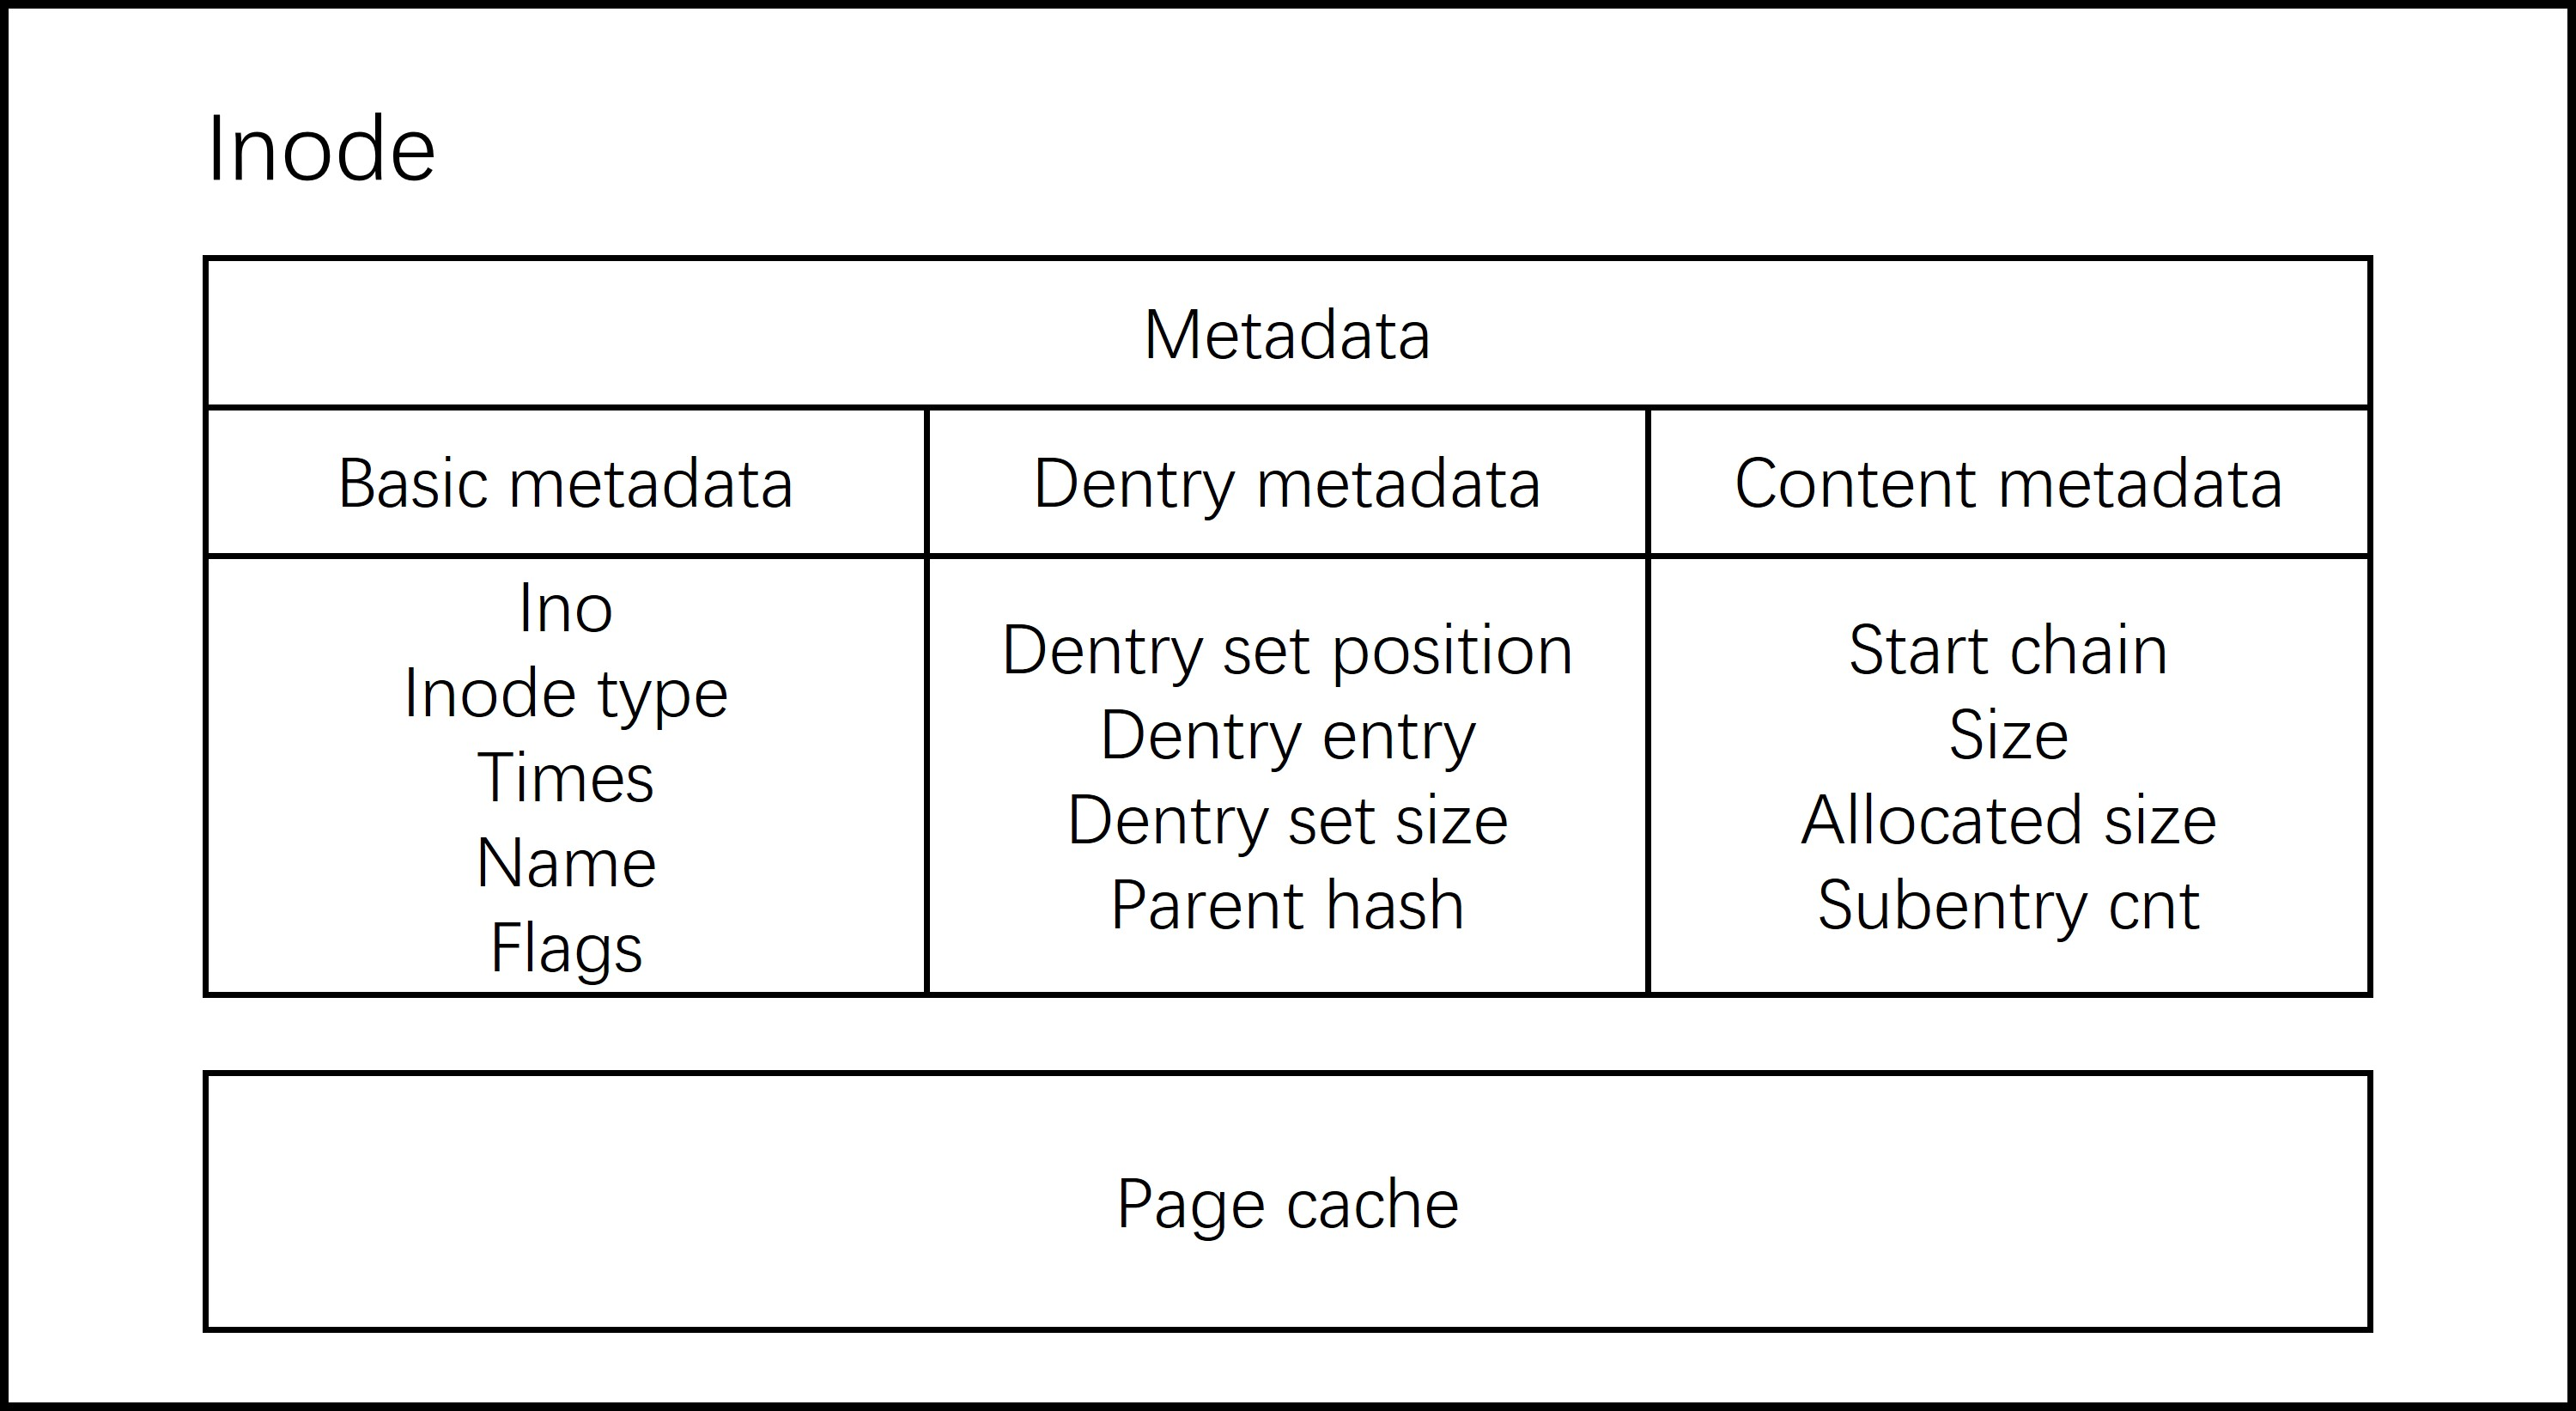
\includegraphics[width=0.8\textwidth]{chap3_inode.jpg}
    \caption{Inode 结构}
    \label{fig:inode}
\end{figure}

我们对 Inode 的设计原则是在能支持完整的文件系统功能的前提下,尽量做到精简,不存储冗余的元数据。
Inode 的结构如图\ref{fig:inode}所示,依据目的不同大致可将 Inode 的成员分为两大类:元数据、页缓存。
其中页缓存用于在内存中缓存文件内容,加速对文件内容的访问。
而元数据又可以按照根据用途不同分为三个主要部分:基本元数据(Basic metadata)、
目录项相关元数据(Dentry metadata)、文件内容元数据(Content metadata)。
下面我们将详细介绍这些元数据。
\begin{itemize}
    \item 基本元数据是和文件的基本信息相关的元数据,包括以下几个部分:
    \begin{itemize} 
        \item 索引节点编号(Ino)
        \item 文件类型(Inode type,可能出现的类型包括文件和目录)
        \item 时间戳(Times,包括创建时间、修改时间、访问时间)
        \item 文件名(Name)
        \item 文件标志位(Flags,描述文件状态,如是否为只读文件等)
    \end{itemize}
    \item 目录项元数据是和文件的目录项集相关的元数据,包括以下几个部分:
    \begin{itemize} 
        \item 目录项集在存储设备上的物理地址(Dentry set position)
        \item 目录项集在其父目录内的逻辑地址(Dentry entry)
        \item 目录项集的大小(Dentry set size)
        \item 父目录 Inode 的哈希值(Parent hash)
    \end{itemize}
    \item 文件内容元数据是和访问文件内容相关的元数据,包括以下几个部分:
    \begin{itemize} 
        \item 文件的起始簇及分配方式(Start chain)
        \item 文件内合法数据的大小(Size)
        \item 文件的分配大小(Allocated size)
        \item 子目录的数量(Subentry cnt,只对目录文件有效)
    \end{itemize}
\end{itemize}

Inode 向上层提供的接口可分为三大类:基本信息接口\ref{tab:basic}、与文件读写相关接口\ref{tab:io}、
与目录操作相关接口\ref{tab:dir}。
每个接口的功能在相应的表格中列出,功能的具体实现主要用到了本章前几节的内容,实现中特别需要注意的点也在对应的描述中标明了。

\begin{table}[h]
    \centering
    \begin{tabularx}{\textwidth}{|c|Y|}
    \hline
    接口 & 描述 \\
    \hline
    ino & 获取 Inode 编号\\
    \hline
    size & 获取文件内合法数据的大小\\
    \hline
    type\_ & 获取文件类型(普通文件、目录等)\\
    \hline
    时间类接口 & 获取或修改时间戳\\
    \hline
    权限相关接口 & 获取或修改文件权限\\
    \hline
    fs & 获取 Inode 所在文件系统引用\\
    \hline
    pagecache & 获取 Inode 内的页缓存引用\\
    \hline
    \end{tabularx}
    \caption{Inode 提供的基本信息接口}
    \label{tab:basic}
\end{table}

\begin{table}[h]
    \centering
    \begin{tabularx}{\textwidth}{|c|Y|}
    \hline
    接口 & 描述 \\
    \hline
    read\_at & 从指定位置读取数据,使用页缓存\\
    \hline
    read\_direct\_at & 从指定位置读取数据,不使用页缓存\\
    \hline
    write\_at & 向指定位置写入数据,使用页缓存\\
    \hline
    write\_direct\_at & 向指定位置写入数据,不使用页缓存\\
    \hline
    resize & 改变文件的分配大小\\
    \hline
    sync & 同步页缓存到存储设备\\
    \hline
    \end{tabularx}
    \caption{Inode 提供的与文件读写相关接口}
    \label{tab:io}
\end{table}

\begin{table}[h]
    \centering
    \begin{tabularx}{\textwidth}{|c|Y|}
    \hline
    接口 & 描述 \\
    \hline
    create & 在当前目录内创建文件或目录,不允许创建同名文件\\
    \hline
    readdir\_at & 从指定位置开始读取当前目录,列出读到的所有文件
    (默认每个目录的前两个条目别是当前目录 . 和父目录 .. )\\
    \hline
    lookup & 在当前目录内查找给定文件名,若存在,返回相应文件的 Inode\\
    \hline
    unlink & 删除当前目录内的指定文件(unlink 是针对非目录文件的接口)\\
    \hline
    rmdir & 删除当前目录内的指定目录(只允许删除空目录)\\
    \hline
    rename & 重命名文件,允许重命名到其他目录下,通过这一点也可以实现文件的移动。
    重命名是一个相对复杂的操作,可以看作是旧目录内删除相应目录项,随后在新目录内创建新的目录项\\
    \hline
    \end{tabularx}
    \caption{Inode 提供的与目录操作相关接口}
    \label{tab:dir}
\end{table}
% vim:ts=4:sw=4

	% Copyright (c) 2014,2016,2018 Casper Ti. Vector
% Public domain.

\chapter{页缓存中数据预取的设计与实现}
%\pkuthssffaq % 中文测试文字。
\section{数据预取的设计}\label{sec:ra_design}
我们的数据预取的设计主要参考了 Linux 系统中的实现\parencite{readahead}。
做数据预取的目的是将磁盘 IO 的延迟对应用程序隐藏,达到应用程序的处理和磁盘 IO 并行的效果。
双窗口 (Dual Windows) 是一种常见的实现手段,可以达成流水线化的数据预取。
如图xx所示,当应用程序在处理当前窗口 (current\_window) 中的数据时,
数据预取在预读窗口 (ahead\_window) 以后台的方式进行。
为了使这种应用程序和磁盘IO并行处理的状态能够延续,我们在 current\_window 中的某个页面上做标记 (lookahead\_index)。
当应用程序访问到带有标记的页面时,便会在预取窗口中触发新的数据预取。
当新的预取操作完成后,窗口会向前推进并在新的窗口内设置新的标记 new\_lookahead\_index。
如此循环往复,也就达到了我们最初的设计目的,表\ref{tab:readahead}总结了设计中的一些关键点。

值得注意的一点是,考虑到数据预取对随机访问模式帮助不大,甚至还可能会起到负面效果,
我们的设计中会检测应用程序的访问模式,只对顺序访问模式做数据预取。
这就涉及到对顺序访问模式的检测,对此我们采用的是一种相对简单的方式:只考虑前一个访问的页面,
如果本次访问的页面编号和前一个访问的页面编号相差不超过1,就认为是本次访问是顺序访问。

\begin{table}[h]
    \centering
    \begin{tabularx}{\textwidth}{|c|Y|}
    \hline
    设计点 & 描述 \\
    \hline
    做预取的时机 & lookahead\_index \\
    \hline
    预取窗口 & readahead\_index .. readahead\_index + size \\
    \hline
    下次预取的时机 & new\_lookahead\_index \\
    \hline
    新的预取窗口 & new\_readahead\_index .. new\_ readahead\_index + new\_size 
                    (new\_readahead\_index = readahead\_index + size)\\
    \hline
    \end{tabularx}
    \caption{数据预取的关键点}
    \label{tab:readahead}
\end{table}

\section{数据预取的实现}
虽然数据预取的设计看起来非常简明,但还有一些实现的细节需要说明。

对于需要维护的状态,我们还是坚持以精简作为设计原则,不维护冗余信息。
为了实现\ref{sec:ra_design}节中的流水线化数据预取,至少需要维护预取窗口和标记页面。
另外,为了支持对应用访问模式的检测,还需要维护前一个访问的页面的编号。

关于预取窗口的长度的设置,我们的实现采用了倍增的方式进行调整。
窗口会被初始化为一个相对小的长度(我们选择了4个页面),随后窗口每向前推进一次,
将窗口大小翻倍,即 $ (offset, size) \Rightarrow (offset + size, 2*size) $。
考虑到底层设备的 IO 请求队列存在上限,为了避免单次请求包含过多的页面,
我们为窗口长度设置了一个上限,一旦达到上限就不再继续倍增。

对于页缓存中的每个页面,有三种可能的状态:未初始化 (Uninit)、已同步 (Sync)、未同步(Dirty),
后两种状态统称为已初始化状态。
页缓存的数据预取属于异步读取,对于异步读取的处理方式一般是,先向存储设备提交读请求并将相关页面
的状态设置为 Uninit,待先前提交的请求完成时,将相关页面的状态更新为 Sync。
另外,为了避免向底层设备提交过多的请求,我们限制最多存在一个未完成的数据预取请求。

图xx是我们为页缓存实现的数据预取算法的伪代码。当上层向页缓存访问编号为 $ idx $ 的页面时,
会调用 $ commit\_page(idx) $。
此时页缓存会首先查看先前提交的预取请求是否完成,如果请求完成,则更新相关页面的状态。
随后,页缓存处理当前访问编号为 $ idx $ 的页面的请求,这可能如下有三种情况。
\begin{itemize}
    \item 情况一:上层请求的页面在页缓存中,并处于已初始化状态。此时请求的页面已经可以返回,
    可以考虑是否提交新的数据预取请求。
    \item 情况二:上层请求的页面在页缓存中,并处于未初始化状态。此时请求的页面属于先前提交的数据预取请求,
    需等待请求的完成,并更新相关页面状态,再考虑是否提交新的数据预取请求。
    \item 情况三:上层请求的页面不在页缓存中。此时不得不做一个同步的读取操作读出请求的页面,
    再考虑是否提交新的数据预取请求。
\end{itemize}
若决定提交新的数据预取请求,则提交请求并初始化相关页面状态,否则直接返回上层请求的页面。

% vim:ts=4:sw=4

	% Copyright (c) 2014,2016,2018 Casper Ti. Vector
% Public domain.

\chapter{实验结果及分析}
%\pkuthssffaq % 中文测试文字。
\section{实验配置}
这一章测试了我们实现的 exFAT 文件系统的性能,并与 Linux 中的对应实现进行了比较。
由于目前 Asterinas 系统还处于开发阶段,还不能实机运行,只能使用 Qemu 进行测试。
故为了确保比较的公平,Linux 的实验结果也是通过 Qemu 取得。
另外,Linux 内核出于某些原因没有预设支持读写 exFAT 文件系统的驱动程序,下面的实验结果是通过 FUSE 套件取得,
可能对性能有一定影响,所以实验结果仅供参考。
我们进行的测试主要目的是测试文件 IO 性能,如果没有特殊说明,测试的默认情景是文件已经存在并且初始化完成,
页缓存在测试开始时为空,在这种情况下通过 FIO 触发文件读写并得到测试结果。
表\ref{tab:exp_setup}总结了本节实验的一些通用配置。

\begin{table}[h]
    \centering
    \begin{tabularx}{\textwidth}{|Y|Y|}
    \hline
    项目 & 描述 \\
    \hline
    存储设备大小 & 4G \\
    \hline
    系统内存大小 & 4G \\
    \hline
    测试文件大小 & 1G \\
    \hline
    单次请求大小 & 4K \\
    \hline
    FIO 测试读写引擎 & sync \\
    \hline
    Linux exFAT套件版本 & FUSE exfat 1.3.0+git20220115 \\
    \hline
    \end{tabularx}
    \caption{实验配置}
    \label{tab:exp_setup}
\end{table}

\section{exFAT文件系统性能测试}\label{sec:exp_file_io}

\begin{figure}[thbp!]
    \centering
    \begin{minipage}[t]{0.49\linewidth}
        \centering
        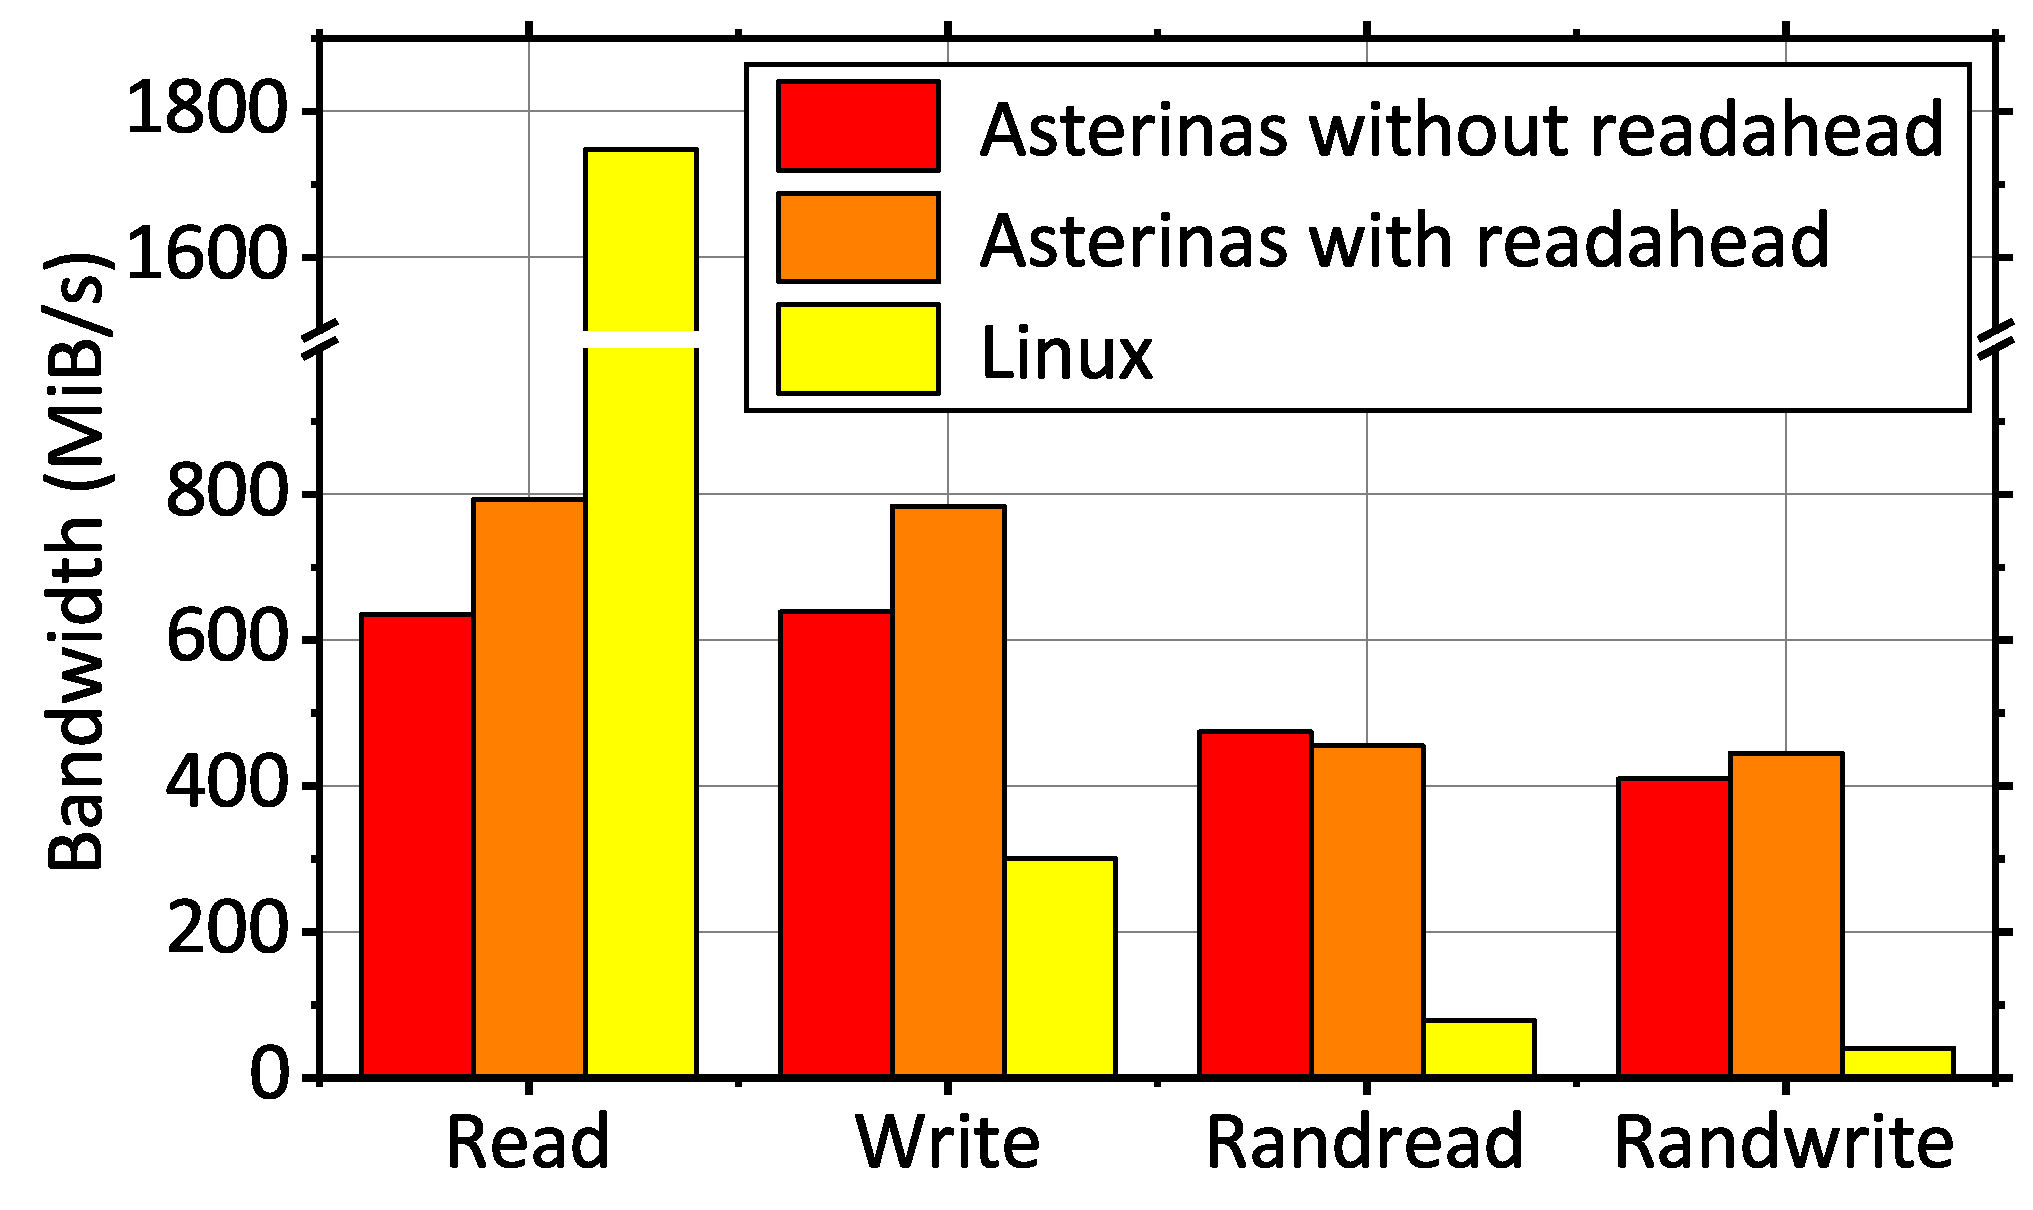
\includegraphics[width=0.9\linewidth]{cached_io.eps}
        \caption{使用页缓存的测试结果}
        \label{fig:cached_io}
    \end{minipage}
    \begin{minipage}[t]{0.49\linewidth}
        \centering
        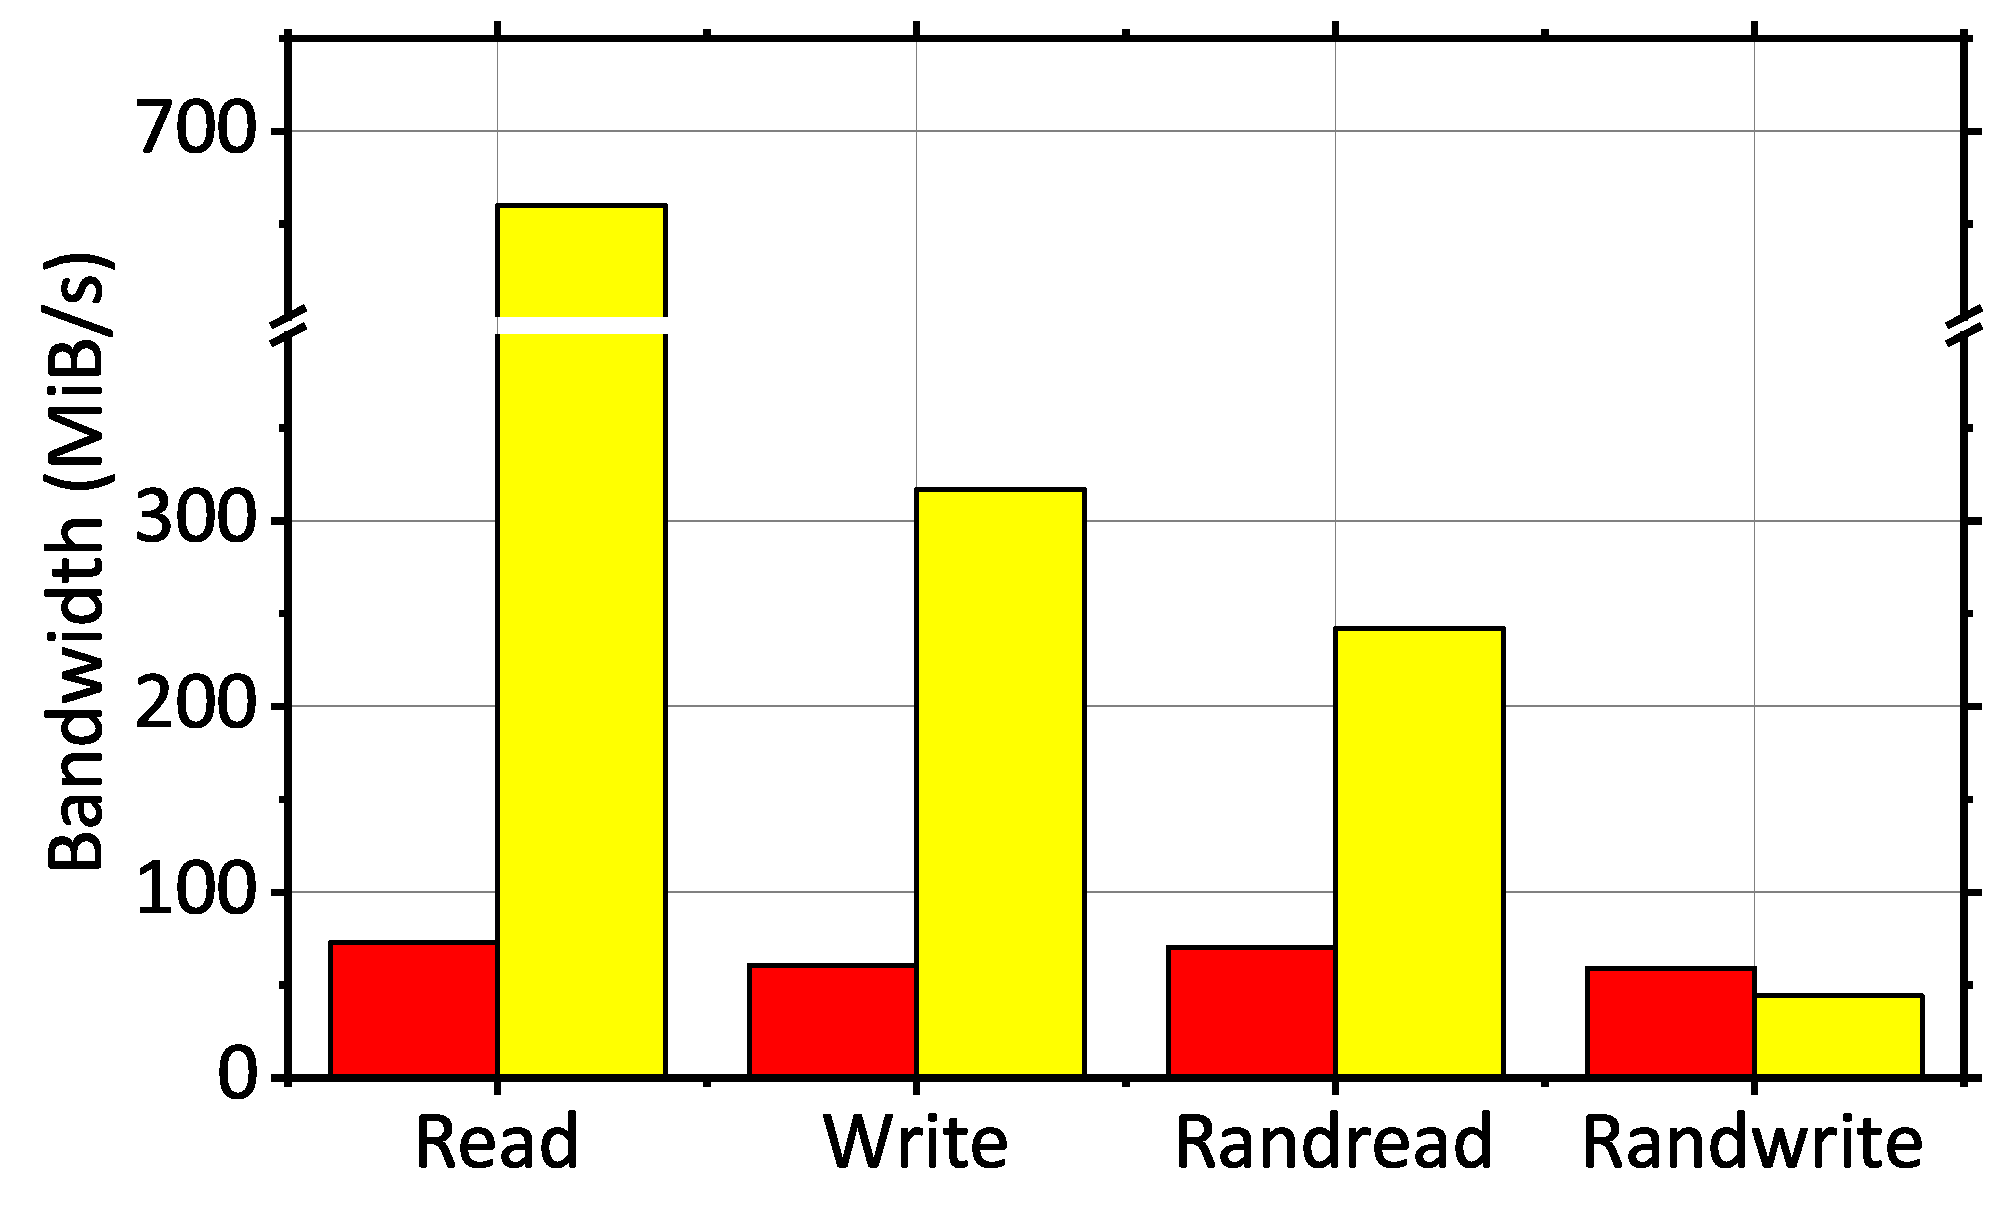
\includegraphics[width=0.9\linewidth]{uncached_io.eps}
        \caption{不使用页缓存的测试结果}
        \label{fig:uncached_io}
    \end{minipage}
 \end{figure}

我们比较了在不同读写模式下,初始页缓存为空的状态下,以单次请求大小为粒度,对测试文件进行连续 60s IO 操作的平均带宽。
图\ref{fig:cached_io}展示了使用页缓存情况下的 IO 带宽,分别比较了使用数据预取的 Asterinas 系统、不使用数据预取的 Asterinas 系统以及 Linux 系统
在顺序读、顺序写、随机读、随机写模式下的 IO 带宽。
图\ref{fig:uncached_io}则展示了不使用页缓存的情况下的 IO 带宽, 仍然是比较了Asterinas 系统(这时是否使用数据预取没有区别)
和 Linux 系统在四种 IO 模式下的带宽。

从图\ref{fig:cached_io}中可以看出,在使用页缓存的情况下,页缓存预取机制的引入提高了顺序访问模式下的 IO 带宽,
而随机访问模式的 IO 带宽没有受到明显影响,整体的 IO 表现符合预期。
此外,通过和 Linux 的对比可以看出,我们的实现在顺序读模式下明显慢于 Linux,但其余 IO 模式都优于 Linux。
考虑到 Linux 的实验结果是通过 FUSE 套件取得,会对性能有一定影响,故这个比较仅供参考。
本节的测试均是连续做 IO 60s 得到的平均性能,从下一节的测试中也能看出,在引入数据预取之后,我们测得的平均性能已经接近峰值性能。
这说明测试文件随着测试的进行会被完全放入页缓存,在这种情况下,因为文件已经被完整缓存,文件系统不会向块设备层发送 IO 新的请求。
但测出的顺序读性能仍然低于 Linux 中的实现,所以页缓存仍有改进的空间。
在不使用缓存的情况下,所有的 IO 均直接与底层块设备进行交互,自然会慢于使用页缓存的结果。
图\ref{fig:uncached_io}中的测试结果表明,Asterinas 系统直接读写块设备的速度普遍慢于 Linux 系统,
这其中可能的原因是测试时的 Asterinas 系统还处于研发初期,其中的块设备层只能支持同步 IO,
而 Linux 系统的块设备层存在异步 IO 以及一些优化策略。

\section{数据预取性能测试}

为了进一步观察我们为页缓存实现数据预取所带来的性能提升,我们又测试了在两种不同的页缓存配置下,使用各种不同的 IO 模式,
对同一文件进行的连续十次相同 IO 的性能变化。
每次 IO 定义为使用相应的读写模式,以单次请求大小为粒度,总计请求和测试文件大小相同的数据。
在第一次 IO 开始前,页缓存是空的,此后的每一次测试都是紧接着前一次测试进行,不清空页缓存。

\begin{figure}[h]
    \centering
    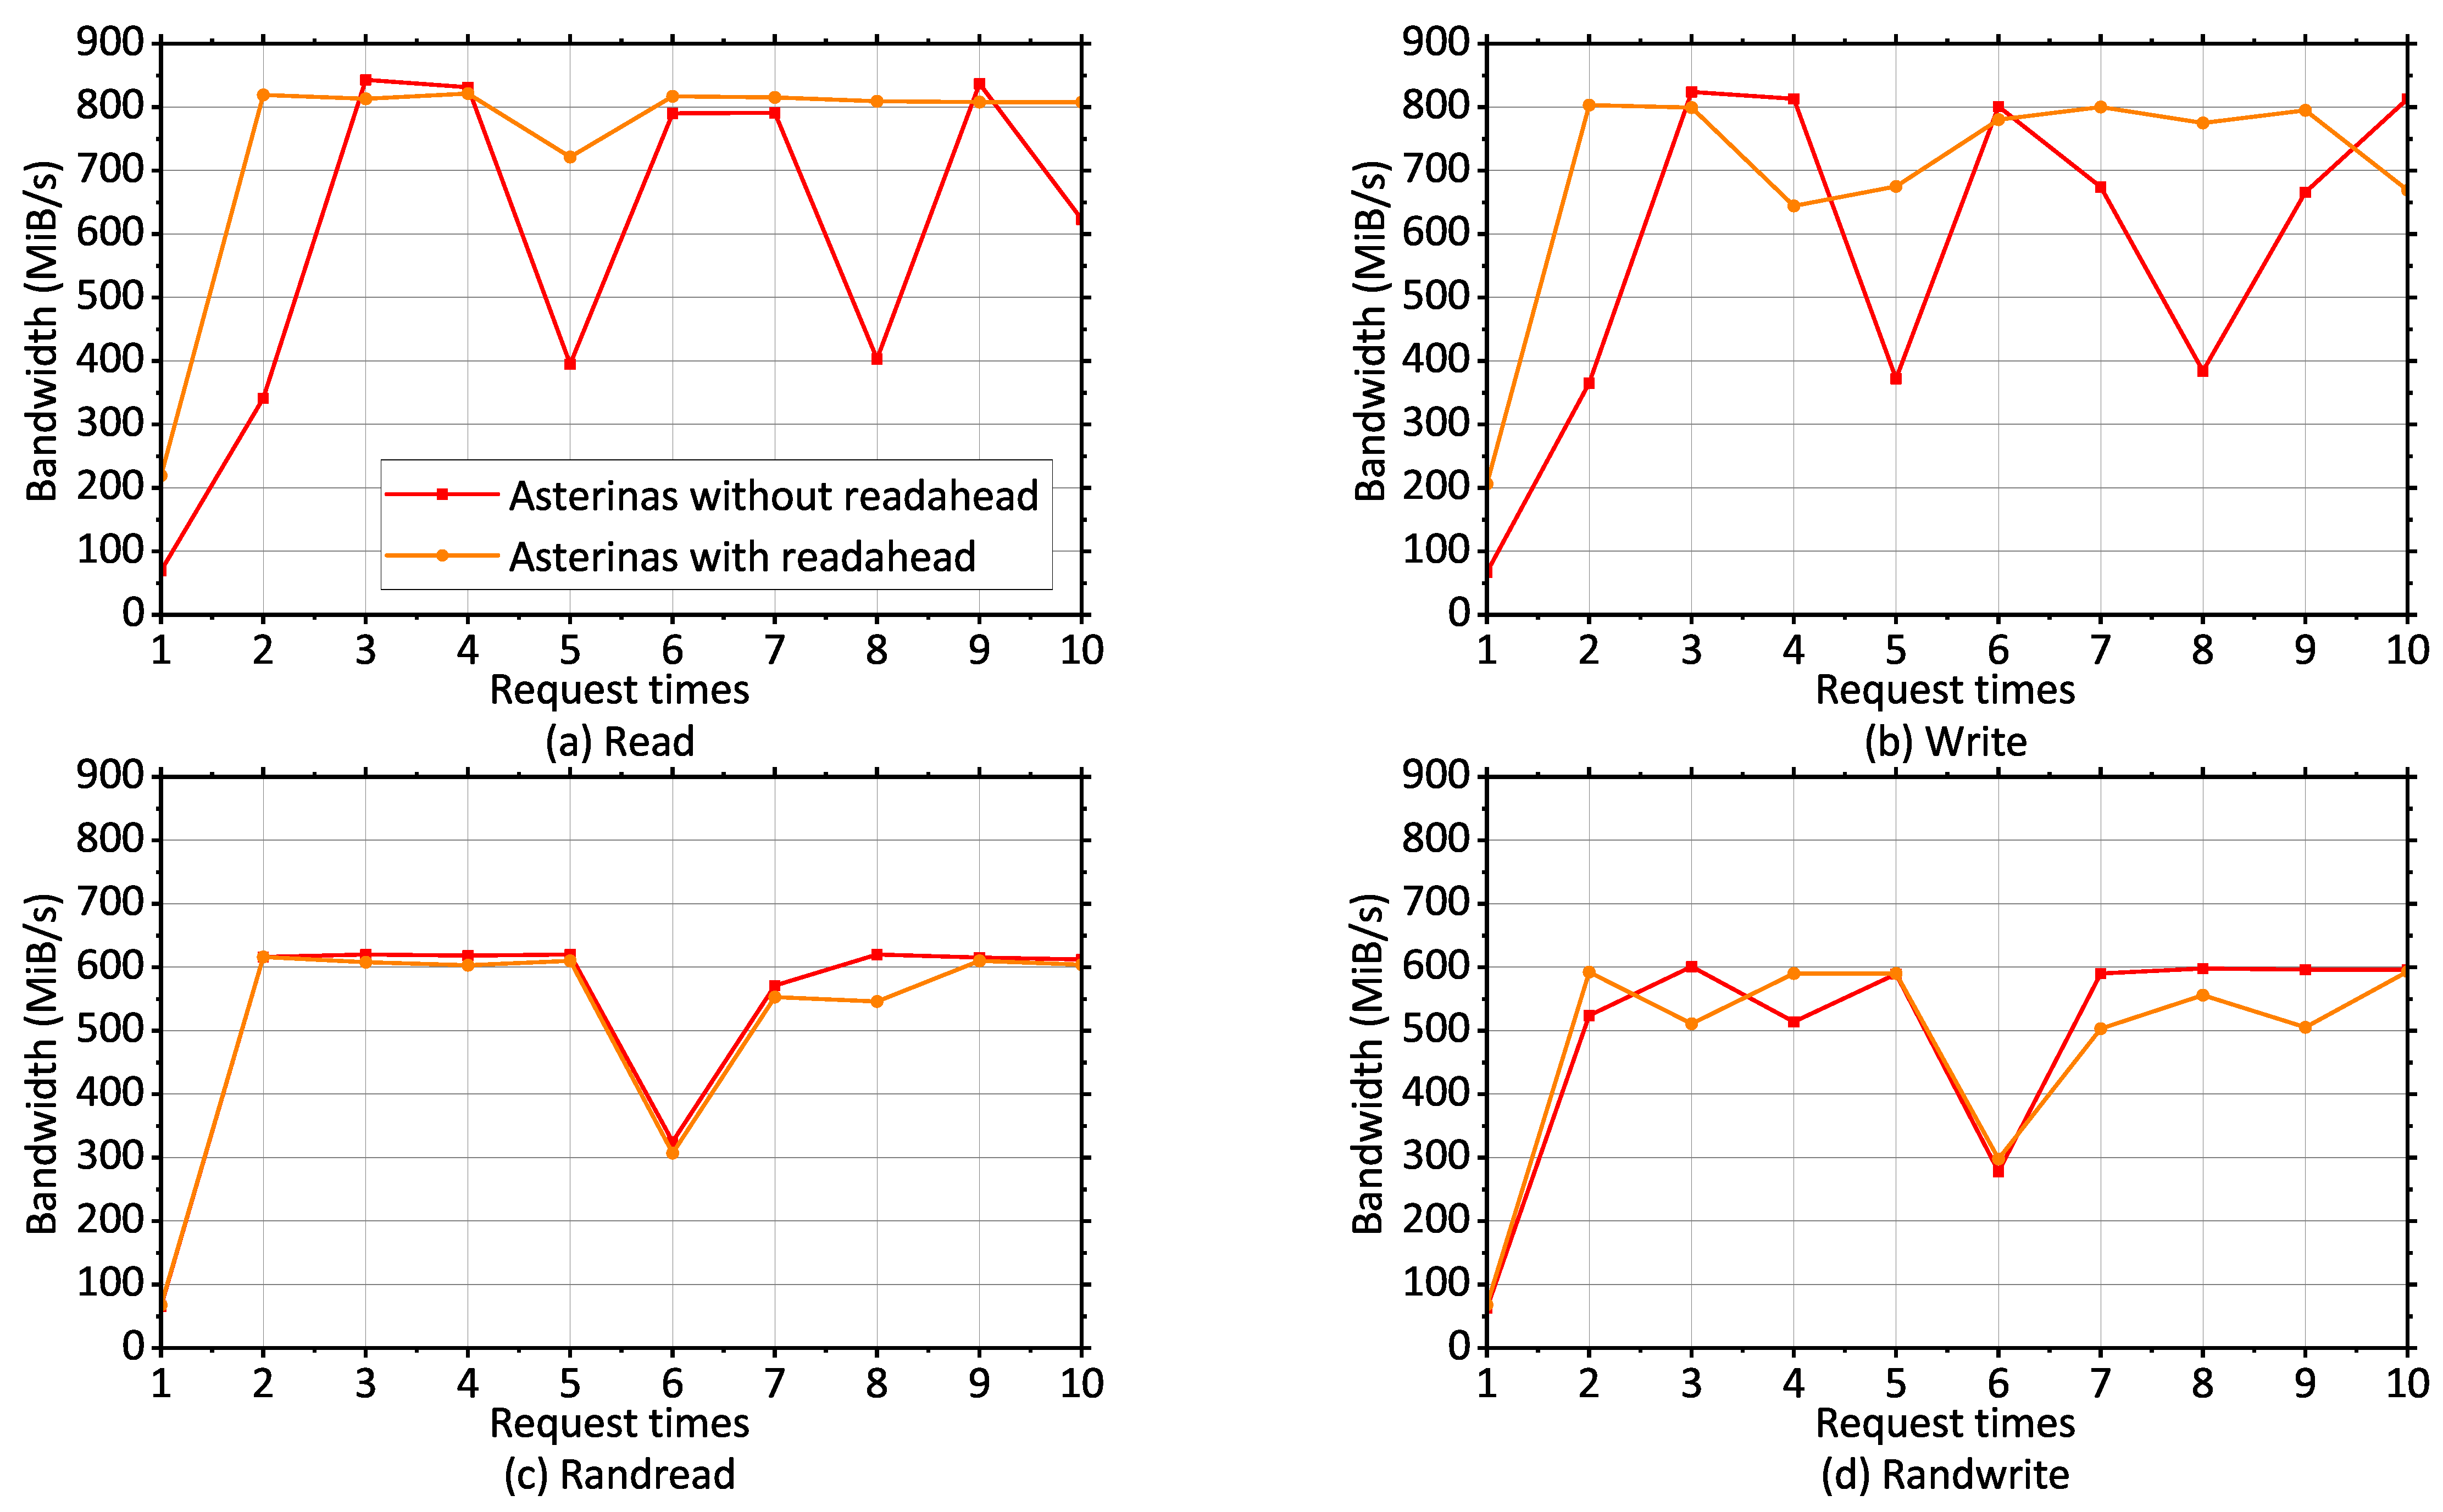
\includegraphics[width=1.0\textwidth]{cmp_combined.eps}
    \caption{使用数据预取与否对性能的影响}
    \label{fig:cmp_ra}
\end{figure}

图\ref{fig:cmp_ra}中展示了我们的测试结果,每张图对应一种 IO 模式,图中的两根曲线分别代表使用数据预取和不使用数据预取的 Asterinas 系统。
从图中可以看出,我们的数据预取的引入主要提升的是顺序 IO 模式的性能表现,对于随机 IO 模式,是否使用数据预取对性能影响不大。
对于顺序 IO 模式,使用数据预取能更快的达到性能峰值,此外,还可以减少性能的波动,使性能维持在峰值附近。
这个结果与\ref{sec:exp_file_io}节的实验结果相符,正是因为 IO 性能能更快的达到峰值,才使得增加数据预取后的总的 IO 性能得到提升。
但从图中还可以看出,我们的数据预取仍有提升的空间,在最理想的情况下顺序 IO 的性能可以在首次调用时便达到峰值,
在这种情况下,上层应用可以完全感知不到块设备层的存在,对于上层应用来说,文件仿佛始终位于内存之中。
这可能是因为测试时 Asterinas 系统的块设备层仍是同步的实现,对此继续改进的方向可能是为块设备层提供异步 IO 支持。
% vim:ts=4:sw=4

	% Copyright (c) 2014,2016,2018 Casper Ti. Vector
% Public domain.

\chapter{结论与展望}
%\pkuthssffaq % 中文测试文字。

% vim:ts=4:sw=4


	% 正文中的附录部分。
	\appendix
	% 排版参考文献列表。bibintoc 选项使“参考文献”出现在目录中;
	% 如果同时要使参考文献列表参与章节编号,可将“bibintoc”改为“bibnumbered”。
	\printbibliography[heading = bibintoc]
	% 各附录。
	% Copyright (c) 2014,2016 Casper Ti. Vector
% Public domain.

\chapter{附件}
\pkuthssffaq % 中文测试文字。
你好哈哈哈哈哈!

% vim:ts=4:sw=4


	% 以下为正文之后的部分,默认不进行章节编号。
	\backmatter
	% 致谢。
	\ifblind\else% Copyright (c) 2014,2016 Casper Ti. Vector
% Public domain.

\chapter{致谢}
%\pkuthssffaq % 中文测试文字。
大学四年已在弹指间呼啸而过,当我回首本科求学的岁月,心中充满感慨与感恩。
首先,我要深深感谢我的父母,你们是我人生道路上最坚实的支柱和最温暖的港湾。
从我蹒跚学步的童年到如今即将毕业的大学生涯,是你们无私的爱和支持,让我始终充满勇气与信心,面对挑战,追求梦想。
每当我陷入迷茫时,是你们的鼓励和信任,让我勇敢前行,勇敢迎接生活的种种考验。
在这里,我想说一声谢谢,谢谢你们给予我的一切。

其次,我要由衷感谢我的导师张杰老师,在我科研迷茫无助之时给予我莫大的帮助。
我接触科研相对同龄人要晚上不少,直到大四才真正进入张杰老师的实验室。
刚进组时,我对科研懵懵懂懂,几乎没有什么科研经历。
但张老师仍对我悉心教导、严格要求,在我科研探索的道路上,您如同一盏明灯,为我指引前行的方向。
在我毕业论文的写作过程中,您不仅给予我耐心的指导和宝贵的建议,更是在学术上给予我无私的帮助。
您的言传身教让我受益匪浅,让我在学术探索的道路上更加坚定和自信。
在此,我要衷心地感谢您,感谢您对我的悉心教导和关怀。

另外,我要特别感谢中关村实验室的闪英迪老师。
在研究期间,闪老师每周都会抽出时间与我开会讨论,给予我细心的指导和莫大的帮助。
您总是在我的项目遇到困难的时候伸出援手,给予我无私的帮助和支持。
没有您的帮助和鼓励,我无法顺利完成毕业论文的写作。
在此,我要衷心地感谢您,感谢您在我求学路上的陪伴和支持。

此外,我还要感谢我的朋友们,特别是我的室友谭亦轩。
在我最需要支持和鼓励的时刻,我的朋友们如同明亮的灯塔,照亮了我前行的道路。
你们不仅是我的知心朋友,更是我生活中最重要的陪伴者和支持者。
在我遭遇挫折时,你们总是第一时间伸出援手,帮助我重新振作,重新勇敢面对生活的挑战。
感谢你们,是你们让我的生活充满了欢笑和温暖,让我在困难中感受到了友情的珍贵。

最后,我要诚挚地感谢所有在我人生中出现的每一个人。
无论是给予建议、支持或批评,你们都是我人生道路上宝贵的财富。
在与你们的相遇中,我学会了成长,学会了坚强,学会了感恩。
谢谢你们,让我在人生的旅途中不再感到孤单,因为有你们的陪伴和支持,让我勇敢面对未来的种种挑战。
感恩有你们,我的大学生涯才如此精彩而难忘。

% vim:ts=4:sw=4
\fi
	% 原创性声明和使用授权说明。
	% Copyright (c) 2008-2009 solvethis
% Copyright (c) 2010-2017,2021 Casper Ti. Vector
% Copyright (c) 2021 Kurapica
% All rights reserved.
%
% Redistribution and use in source and binary forms, with or without
% modification, are permitted provided that the following conditions are
% met:
%
% * Redistributions of source code must retain the above copyright notice,
%   this list of conditions and the following disclaimer.
% * Redistributions in binary form must reproduce the above copyright
%   notice, this list of conditions and the following disclaimer in the
%   documentation and/or other materials provided with the distribution.
% * Neither the name of Peking University nor the names of its contributors
%   may be used to endorse or promote products derived from this software
%   without specific prior written permission.
%
% THIS SOFTWARE IS PROVIDED BY THE COPYRIGHT HOLDERS AND CONTRIBUTORS "AS
% IS" AND ANY EXPRESS OR IMPLIED WARRANTIES, INCLUDING, BUT NOT LIMITED TO,
% THE IMPLIED WARRANTIES OF MERCHANTABILITY AND FITNESS FOR A PARTICULAR
% PURPOSE ARE DISCLAIMED. IN NO EVENT SHALL THE COPYRIGHT HOLDER OR
% CONTRIBUTORS BE LIABLE FOR ANY DIRECT, INDIRECT, INCIDENTAL, SPECIAL,
% EXEMPLARY, OR CONSEQUENTIAL DAMAGES (INCLUDING, BUT NOT LIMITED TO,
% PROCUREMENT OF SUBSTITUTE GOODS OR SERVICES; LOSS OF USE, DATA, OR
% PROFITS; OR BUSINESS INTERRUPTION) HOWEVER CAUSED AND ON ANY THEORY OF
% LIABILITY, WHETHER IN CONTRACT, STRICT LIABILITY, OR TORT (INCLUDING
% NEGLIGENCE OR OTHERWISE) ARISING IN ANY WAY OUT OF THE USE OF THIS
% SOFTWARE, EVEN IF ADVISED OF THE POSSIBILITY OF SUCH DAMAGE.

{
	\ctexset{section = {
		format+ = {\centering}, beforeskip = {40bp}, afterskip = {15bp}
	}}
	\specialchap{北京大学学位论文原创性声明和使用授权说明}

	% 学校书面要求本页面不要页码,但在给出的 Word 模版中又有页码。
	% 此处以学校书面要求为准。
	\thispagestyle{empty}
	\mbox{}\vspace*{-3em}
	\section*{原创性声明}

	本人郑重声明:
	所呈交的学位论文,是本人在导师的指导下,独立进行研究工作所取得的成果。
	除文中已经注明引用的内容外,
	本论文不含任何其他个人或集体已经发表或撰写过的作品或成果。
	对本文的研究做出重要贡献的个人和集体,均已在文中以明确方式标明。
	本声明的法律结果由本人承担。
	\vskip 1em
	\rightline{%
		论文作者签名:\hspace{9em}
	}
	\rightline{% \\
		日期:\hspace{2em}年\hspace{2em}月\hspace{2em}日%
	}

	\section*{%
		学位论文使用授权说明\\[-0.33em]
	}

	本人完全了解北京大学关于收集、保存、使用学位论文的规定,即:
	\begin{itemize}
		\item 按照学校要求提交学位论文的印刷本和电子版本;
		\item 学校有权保存学位论文的印刷本和电子版,
			并提供目录检索与阅览服务,在校园网上提供服务;
		\item 学校可以采用影印、缩印、数字化或其它复制手段保存论文;
	\end{itemize}
	\vskip 1em
	\rightline{%
		论文作者签名:\hspace{5em}导师签名:\hspace{5em}
	}
	\rightline{% \\
		日期:\hspace{2em}年\hspace{2em}月\hspace{2em}日\hspace{6em}%
	}

	% 若须排版二维码,请将二维码图片重命名为“barcode”,
	% 转为合适的图片格式,并放在当前目录下,然后去掉下面 2 行的注释。
	%\vfill\noindent
	%\includegraphics[height = 5em]{barcode}
}

% vim:ts=4:sw=4

\end{document}

% vim:ts=4:sw=4
